\chapter{Introduction}
%\addstarredchapter{Introduction}
%\markboth{Introduction}{Introduction}
\label{chap:introduction}
%\minitoc

Les phénomènes physiques peuvent être extrêmement variés, allant de la propagation des ondes dans un milieu, aux écoulements de fluides, à la diffusion de la chaleur, aux vibrations des structures, aux phénomènes électromagnétiques, etc. La modélisation mathématique consiste à représenter ces phénomènes sous forme de relations, en utilisant des équations et des concepts appropriés. L'objectif est de comprendre le comportement du système étudié, de prédire son évolution dans le temps et dans l'espace, et éventuellement de prendre des décisions éclairées en fonction des résultats obtenus.\\

La modélisation mathématique aboutit souvent à l'obtention d'équations aux dérivées partielles (EDP) qui sont un outil fondamental en mathématiques appliquées pour la modélisation des phénomènes physiques. Elles permettent de décrire et d'analyser des systèmes dynamiques complexes en prenant en compte les variations spatio-temporelles des grandeurs physiques. Ces équations aux dérivées partielles expriment les relations entre les dérivées partielles des variables impliquées, telles que la position, le temps, la température, la pression, la vitesse, etc. Elles capturent ainsi les comportements changeants des phénomènes physiques et permettent de formuler des modèles mathématiques précis pour les étudier.\\

La résolution des équations aux dérivées partielles peut se faire de différentes manières. Dans certains cas, il est possible d'obtenir des solutions analytiques exactes, qui fournissent une compréhension profonde du système étudié. Cependant, la plupart du temps, ces équations sont si complexes qu'il est nécessaire d'utiliser des méthodes numériques pour les résoudre de manière approximative. Ces méthodes impliquent la discrétisation de l'espace et du temps, et la transformation des équations en un système d'équations aux différences ou aux intégrales. Ces systèmes sont ensuite résolus numériquement à l'aide d'algorithmes appropriés, permettant d'obtenir des solutions numériques qui approchent la réponse du système réel.


\section{Méthodes numériques pour la résolution d'EDP}

Les méthodes numériques de résolution des équations aux dérivées partielles (EDP) sont des approches mathématiques utilisées pour obtenir des approximations des solutions de ces équations sur des domaines discrétisés.

\subsection{Quelques schémas numériques}

L'une des méthodes numériques les plus couramment utilisées pour résoudre les EDP est la méthode FD pour \emph{Finite Difference} \cite{forsythe1961finite, smith1985numerical, stummel2006difference}. Cette méthode consiste à discrétiser l'espace et le temps, en remplaçant le domaine continu par une grille de points discrets. Les dérivées spatiales et temporelles sont ensuite approximées à l'aide d'opérateurs de différences finies. Les équations aux dérivées partielles sont transformées en un système d'équations algébriques, qui peut être résolu numériquement à l'aide de techniques d'algèbre linéaire.

Une autre méthode numérique couramment utilisée est la méthode FEM pour \emph{Finite Element Method} \cite{zienkiewicz2005finite, norrie2014finite}. Cette méthode repose sur la discrétisation du domaine continu en éléments finis, tels que des triangles ou des quadrilatères pour les problèmes en deux dimensions, ou des tétraèdres ou des hexaèdres pour les problèmes en trois dimensions. Les fonctions de base sont définies sur ces éléments finis, et la solution de l'EDP est approximée par une combinaison linéaire de ces fonctions de base. Le problème continu est alors transformé en un système d'équations linéaires.

Les méthodes FV pour \emph{Finite Volume} \cite{leveque2002finite, barth2003finite} constituent une autre approche couramment utilisée pour résoudre les EDP. Elles consistent à discrétiser le domaine en volumes, tels que des cellules polyhédrales, et à approximer les flux à travers les interfaces des volumes. Les schémas FV se base sur une écriture sous forme conservative des équations permettant de faire apparaître le flux, par la suite discrétisé en utilisant des schémas de flux numériques, tels que le schéma de Lax-Friedrichs ou le schéma de Roe.

La méthode DG pour \emph{Discontinuous Galerkin} \cite{arnold2000discontinuous, riviere2008discontinuous} combine des aspects de la méthode des éléments finis et des méthodes de volumes finis. Elle consiste à diviser le domaine en éléments finis et à approximer la solution par des fonctions discrètes définies localement sur chaque élément. Contrairement à la méthode des éléments finis, la méthode DG permet des discontinuités de la solution entre les éléments. Les flux entre les éléments sont pris en compte par des termes de saut, qui sont intégrés dans le système d'équations. Cette méthode permet d'obtenir une montée en ordre dans les schémas FV sur le même principe que pour les FE d'ordre élevé.

Les méthodes SD pour \emph{Spectral Difference} sont des méthodes numériques basées sur l'approximation des dérivées partielles à l'aide de fonctions de base spectrale \cite{liu2006spectral, van2008stability}. Elles utilisent des polynômes ou des séries de fonctions orthogonales pour représenter la solution de manière très précise et comme pour les FD décrivent une approximation forte des EDP. Les différences spectrales offrent une convergence rapide et une haute précision pour les solutions régulières. Cependant, elles peuvent être plus complexes à mettre en œuvre et nécessitent souvent des grilles régulières pour optimiser les performances.

%La méthode des éléments spectraux est une extension de la méthode des éléments finis qui utilise des fonctions de base spectrales pour représenter la solution. Elle permet une convergence rapide et une précision élevée, même avec un petit nombre d'éléments, en particulier pour les problèmes avec des solutions régulières. La méthode des éléments spectraux peut être combinée avec des techniques d'optimisation pour obtenir des solutions optimales ou pour résoudre des problèmes inverse.

La méthode BEM pour \emph{Boundary Element Method}, également connue sous le nom de méthode des éléments de frontière, est une méthode numérique qui se concentre sur la discrétisation de la frontière du domaine plutôt que sur l'intérieur \cite{nedelec2001acoustic, wu2002boundary, kirkup2019boundary}. Elle permet de réduire la dimension du problème en transformant l'EDP en une équation intégrale définie sur la frontière ensuite approchée par une représentation FE. Cette méthode se révèle particulièrement avantageuse pour les situations où la géométrie du problème est bidimensionnelle, car elle permet d'éviter la complexité liée à la discrétisation de l'intérieur du domaine. De plus, elle est particulièrement efficace lorsque la solution est régulière le long de la frontière.\\

Toutes ces méthodes numériques partagent un point commun fondamental : la discrétisation du domaine de calcul. En effet, pour pouvoir effectuer des calculs numériques sur ordinateur, il est nécessaire de représenter le domaine continu par un maillage discret. La discrétisation du domaine consiste à subdiviser l'espace en un ensemble fini de points, d'éléments ou de volumes de contrôle. Cette subdivision permet de représenter le problème continu sous une forme discrète, ce qui facilite la résolution numérique. En décomposant le domaine en éléments discrets, on réduit la complexité du problème et on le transforme en un ensemble de calculs dénombrables (finis). Le maillage utilisé peut prendre différentes formes en fonction de la nature du problème et des exigences spécifiques.


\subsection{Influence du maillage}

Le choix du maillage et sa qualité ont un impact significatif sur la précision, la stabilité, l'efficacité et l'exactitude des résultats numériques obtenus. Dans cette partie, nous explorons l'influence du maillage sur les schémas numériques utilisés pour résoudre des problèmes physiques en sciences et en ingénierie.

\subsubsection{Précision de la solution}

La question de la précision des résultats dans le contexte de la modélisation numérique est étroitement liée à la qualité du maillage utilisé. Un maillage finement discretisé offre une représentation plus fidèle de la géométrie sous-jacente et des variations spatiales des phénomènes analysés. Cette approche permet de capturer de manière plus précise les gradients élevés présents dans les solutions, ce qui se traduit par des résultats numériques d'une plus grande exactitude. Par exemple, dans la simulation de fluides, un maillage fin peut mieux représenter les tourbillons et les interactions complexes entre les particules fluides. De même, dans la modélisation de structures, un maillage fin peut aider à capturer les déformations locales avec une plus grande précision.

À l'opposé, l'utilisation d'un maillage grossier peut introduire des erreurs substantielles dans les solutions numériques. En effet, les variations spatiales et les détails géométriques sont sous-représentés dans un maillage grossier, ce qui peut conduire à des estimations biaisées ou incorrectes des phénomènes étudiés. Les gradients élevés ne sont pas correctement résolus, ce qui peut aboutir à des approximations inexactes et des prédictions éloignées des véritables comportements.


\subsubsection{Temps de calcul}

Un des défis incontournables de la modélisation numérique réside dans la gestion des temps de calcul, qui est étroitement liée au nombre d'inconnues à calculer, proportionnel au nombre de cellules. En effet, la finesse du maillage peut avoir un impact significatif sur la durée nécessaire pour effectuer les simulations, en particulier pour les problèmes en trois dimensions.

Pour résoudre le dilemme entre précision et temps de calcul, une variété d'approches peuvent être envisagées. L'une de ces approches repose sur l'adaptation de maillage, consistant à accroître la résolution dans les régions d'intérêt tout en conservant un maillage moins détaillé dans les zones moins critiques. En complément, les techniques de parallélisation se montrent efficaces pour répartir la charge de calcul sur plusieurs processeurs, entraînant une accélération du temps de résolution global. En outre, la réduction du nombre de degrés de liberté contribue à diminuer les coûts mémoire.

\subsubsection{Adaptation du maillage}

L'adaptation du maillage représente une avancée significative dans le domaine de la modélisation numérique, offrant une approche dynamique pour résoudre efficacement et précisément des problèmes complexes. Les maillages adaptatifs apportent une réponse ingénieuse aux défis posés par des phénomènes variés et hétérogènes en ajustant automatiquement la taille et la distribution des éléments du maillage en fonction des caractéristiques locales du système étudié. L'idée sous-jacente à l'adaptation du maillage est d'assigner davantage de ressources numériques là où elles sont le plus nécessaires pour capturer les détails importants du phénomène. Plutôt que d'utiliser un maillage uniforme, les maillages adaptatifs identifient les zones où des variations significatives se produisent, telles que des gradients élevés de variables physiques ou des interfaces entre différentes phases. En conséquence, les éléments du maillage sont raffinés dans ces régions d'intérêt, permettant une représentation plus fine et plus précise du phénomène, tandis que les régions moins critiques sont traitées avec des éléments plus gros, réduisant ainsi le coût global du calcul.

L'impact positif de cette approche est multiple. Tout d'abord, elle permet de réaliser des simulations plus efficaces en concentrant les ressources de calcul là où elles sont les plus nécessaires. Cela se traduit par des temps de calcul réduits, car les régions moins dynamiques ne nécessitent pas autant de détails pour obtenir une solution précise. Deuxièmement, l'adaptation du maillage améliore la qualité des résultats. Les détails locaux, tels que les chocs ou les frontières complexes, sont mieux capturés, renforçant la validité physique des simulations.

\subsubsection{Stabilité du schéma numérique}

La stabilité des schémas numériques joue un rôle crucial dans la précision des résultats obtenus lors de simulations numériques. Il convient de noter que cette notion peut être étroitement liée à la taille des éléments du maillage utilisé. Certains schémas numériques, connus sous le nom de schémas conditionnellement stables, présentent une particularité: leur stabilité dépend de la taille du pas de temps et des dimensions des éléments de maillage. Si la taille du pas de temps est choisie de manière inappropriée ou si le maillage est trop fin, cela peut conduire à des instabilités numériques, générant des résultats non convergents ou incorrects.

D'un point de vue pratique, cela signifie que même si l'utilisation d'un maillage fin puisse potentiellement permettre une capture précise des détails géométriques et des variations spatiales, il est essentiel de prendre soigneusement en compte la stabilité du schéma numérique. La forme des éléments et l'inhomogénéité du maillage ont un impact direct sur le nombre de CFL, et le choix d'un pas de temps approprié par rapport à la taille du maillage peut devenir une tâche complexe, impliquant des compromis entre la précision des résultats et la stabilité numérique.


\subsubsection{Conservation des propriétés physiques}

Généralement la modélisation numérique reposent sur la préservation des lois fondamentales de la physique, telles que la conservation de la masse, de l'énergie et de la quantité de mouvement. Ces propriétés jouent un rôle crucial dans la précision et la validité des simulations numériques. Cependant, le choix d'un maillage inadéquat peut entraîner des conséquences néfastes. Des erreurs numériques peuvent surgir, altérant la conservation de ces propriétés physiques cruciales.

Considérons par exemple un fluide en mouvement dans une simulation. Si le maillage n'est pas adapté, il pourrait ne pas représenter correctement les gradients de vitesse, ce qui résulterait en une violation de la conservation de la quantité de mouvement. Cela signifierait que la simulation ne tiendrait pas compte de la manière dont le fluide interagit avec les forces extérieures et ne reproduirait pas fidèlement les comportements réels. De même si les cellules du maillage sont mal positionnées ou de tailles inégales, cela pourrait conduire à une mauvaise estimation des densités et donc à une non-conservation de la masse.


\subsubsection{Parallélisation}

La manière dont le maillage est structuré et organisé peut jouer un rôle crucial dans la parallélisation des calculs numériques, en particulier pour les méthodes qui reposent sur des maillages structurés. La parallélisation est une stratégie clé pour accélérer les simulations numériques en divisant les calculs en plusieurs tâches indépendantes pouvant être exécutées simultanément sur différents processeurs ou cœurs de calcul.

Lorsque le maillage est conçu de manière à ce que les éléments voisins partagent des caractéristiques similaires, il devient plus simple d'assigner des groupes d'éléments à différents processeurs. Cette organisation permet aux processeurs de travailler sur des parties du maillage qui sont cohérentes en termes de calculs et de communications nécessaires, minimisant ainsi les temps d'attente et les transferts de données inutiles. En revanche, si les éléments du maillage sont de tailles très différentes ou si les interactions entre éléments sont incohérentes, la répartition des tâches entre les processeurs peut devenir déséquilibrée. Certains processeurs pourraient être surchargés de calculs complexes tandis que d'autres restent inactifs, ce qui réduit l'efficacité globale de la parallélisation.

Un autre aspect important est la manière dont les données sont échangées entre les processeurs lors de la parallélisation. Un maillage bien structuré peut minimiser les besoins en communications entre les processeurs, car les éléments voisins sont susceptibles de nécessiter moins d'échanges de données. Cela réduit les goulots d'étranglement et améliore la vitesse d'exécution globale.

\subsubsection{Intégration dans des géométries complexes}

Un exemple concret de l'importance de l'intégration des problèmes numériques dans des géométries complexes se trouve dans la simulation de flux de fluides à travers des réseaux de canaux sinueux. Considérons un système de canalisations dans une installation industrielle ou un réseau de vaisseaux sanguins dans le corps humain, où les canaux peuvent avoir des formes tortueuses, des embranchements multiples et des variations géométriques importantes.

Pour résoudre numériquement le comportement des fluides dans ces canaux, il est essentiel de créer un maillage adapté qui représente fidèlement la géométrie complexe. Un maillage de qualité médiocre pourrait entraîner des inexactitudes significatives dans la prédiction des propriétés du flux, telles que la pression, la vitesse et les gradients de concentration.

La création d'un maillage approprié pour ce type de géométrie complexe peut nécessiter des techniques spécialisées, telles que la génération de maillage à l'aide de méthodes basées sur les équations d'advection-diffusion pour les canaux, ou l'utilisation de techniques de maillage adaptatif pour concentrer la résolution là où les variations du flux sont les plus importantes. De plus, la méthode des éléments finis de frontière pourrait être employée pour simplifier le maillage en ne le construisant qu'à la frontière des canaux.\\

\begin{comment}
    \paragraph{Diffusion numérique :}
    La diffusion numérique est un effet indésirable qui peut se produire avec certains schémas numériques. Un maillage adapté avec une bonne résolution spatiale peut réduire la diffusion numérique en permettant une meilleure capture des gradients et des phénomènes rapides.
    
    \paragraph{Exactitude du modèle :}
    Un maillage fin et adapté peut améliorer la précision et l'exactitude du modèle numérique en le rapprochant des résultats expérimentaux ou des solutions analytiques connues. Un maillage inapproprié peut entraîner des divergences significatives entre les résultats numériques et les données réelles.
    
    \paragraph{Effets de bord :}
    Un maillage de mauvaise qualité peut provoquer des effets de bord indésirables, tels que des réflexions parasites, des interférences ou des perturbations artificielles dans les résultats numériques. Un maillage plus fin peut aider à réduire ces effets, mais il est essentiel de choisir un maillage approprié pour minimiser ces problèmes.
\end{comment}

Un maillage bien choisi et bien conçu est essentiel pour obtenir des résultats numériques fiables et représentatifs des phénomènes réels. En considérant les aspects de précision, de stabilité, d'efficacité et d'exactitude, ainsi que les défis liés aux géométries complexes, les scientifiques et les ingénieurs peuvent améliorer la qualité et la pertinence de leurs simulations numériques grâce à une approche réfléchie du maillage. Dans la suite, nous explorerons les avantages spécifiques des maillages quadrilatéraux qui en font un choix privilégié dans de nombreux cas.

\subsection{Intérêts des maillages quadrilatéraux}

La plupart des schémas numériques utilisés pour la simulation sont basés sur une discrétisation (le maillage) du domaine de calcul englobant la scène que l'on souhaite modéliser. Les différents schémas connus se basent alors sur un type de maillage donné présentant un intérêt propre : différences Finies sur maillages cartésiens pour la simplicité et l'efficacité, éléments Finis sur maillages conformes (triangles ou tétraèdres) pour la bonne représentation des objets, méthodes isoparamétriques sur maillages courbes pour le rendu près d'effets proches de parois complexes, volumes Finis ou Galerkin discontinu sur maillages non-structurés et conformes pour introduire des raffinements locaux etc.

Les outils de générations de maillage pour les codes de simulation numérique se sont alors grandement développés. Pour autant, au sein d'une même famille de schémas, il est possible d'obtenir des résultats extrêmement différents, aussi bien en qualité qu'en efficacité, selon les fonctions de base choisies et donc selon les éléments utilisés. Ainsi, sur un certain nombre de schémas hautes précision (Galerkin discontinu, éléments finis d'ordre élevés, différences finies spectrales etc.) on observe que les fonctions de bases définies sur quadrilatères en 2D, ou hexaèdres en 3D, présentent d'excellentes propriétés développées ci-après.

\subsubsection{Régularité/ Structuration}

Les maillages de type quadrilatéral se caractérisent par une régularité intrinsèque qui les rapproche de structures de grilles ordonnées. Cette particularité leur confère divers avantages majeurs dans le contexte des simulations numériques fondées sur la méthode des éléments finis. Une mise en lumière excellente de plusieurs de ces avantages peut être trouvée dans la thèse de Maxence Reberol \cite{reberol2018maillages}.

L'un des atouts majeurs dans ce cadre réside dans la capacité de prévoir à l'avance la largeur de bande des matrices clairsemées employées dans les calculs. Cette propriété revêt une importance cruciale pour les systèmes linéaires intégrés aux méthodes numériques, car elle permet d'optimiser l'utilisation des ressources de calcul et de réduire les coûts de stockage. En contraste, les maillages triangulaires, en raison de leur nature fondamentalement non structurée, ne permettent pas une anticipation aussi aisée de la bande utile de la matrice. Cette complexité dans la prévision de la bande conduit à une gestion plus délicate et à des besoins de stockage fréquemment plus élevés. De plus, il est possible de maintenir une largeur de bande constante ce qui permet d'exploiter pleinement les performances des algorithmes de produits matrices-vecteurs, tirant parti des capacités de calcul parallèle des processeurs.

Une autre qualité bénéfique des maillages quadrilatéraux structurés est liée à la gestion des informations de connectivité entre les éléments du maillage. Par le biais d'une numérotation appropriée, il devient envisageable d'éviter le stockage explicite de ces connexions, car elles peuvent être déduites de manière implicite. Cette approche entraîne des économies significatives en matière de stockage et d'accès mémoire, ce qui revêt une importance capitale pour les simulations numériques de grande envergure utilisant des maillages complexes.

%Dans le contexte des méthodes numériques, l'efficacité des maillages structurés prend toute son importance, en particulier dans des domaines tels que la méthode de Galerkine discontinue. Dans cette variante, la différence entre les maillages quadrilatéraux structurés et les maillages triangulaires non structurés peut avoir un impact significatif sur la précision et la rapidité des calculs. Alors que la méthode classique des éléments finis peut avoir un temps de calcul similaire dans les deux cas, les maillages structurés se révèlent souvent bien plus performants et offrent un meilleur rapport précision-temps de calcul dans ces variantes plus exigeantes.

\subsubsection{$\mathbb{P}_k$ vs $\mathbb{Q}_k$}

\'Etant donné un maillage $\mathcal{T}_h$ d'un ouvert connexe polyédrique $\Omega\subset\mathbb{R}^N$, la méthode des éléments finis $\mathbb{P}_k$ \cite{allaire2005analyse}, associée à ce maillage, est définie par l'espace discret:
$$V_h=\{v\in C(\bar{\Omega)}\text{ tel que }v|_{K}\in\mathbb{P}_k\text{ pour tout }K\in\mathcal{T}_h\}$$
où $\mathbb{P}_k$ est l'ensemble des polynômes à coefficients réels de $\mathbb{R}^N$ dans $\mathbb{R}$ de degré inférieur ou égal à $k$, c'est à dire que pour tout $p\in\mathbb{P}_k$,
$$p(x)=\displaystyle\sum_{i_1,\dots, i_N\geq 0\atop i_1+\dots+i_N\leq k}\alpha_{i_1,\dots,i_N}x_1^{i_1}\dots x_N^{i_N}\text{ avec }x=(x_1,\dots,x_N),$$
tandis que la méthode des éléments finis $\mathbb{Q}_k$ est définie par l'espace discret:
$$V_h=\{v\in C(\bar{\Omega)}\text{ tel que }v|_{K}\in\mathbb{Q}_k\text{ pour tout }K\in\mathcal{T}_h\}$$
où $\mathbb{Q}_k$ est l'ensemble des polynômes à coefficients réels de $\mathbb{R}^N$ dans $\mathbb{R}$ de degré inférieur ou égal à $k$ \textbf{par rapport à chaque variable}, c'est à dire que pour tout $q\in\mathbb{Q}_k$,
$$q(x)=\displaystyle\sum_{0\leq i_1\leq k,\dots,0\leq i_N\leq k}\alpha_{i_1,\dots,i_N}x_1^{i_1}\dots x_N^{i_N}\text{ avec }x=(x_1,\dots,x_N).$$
Les éléments $\mathbb{P}_k$ présentent un nombre de degrés de liberté en adéquation avec la forme des triangles, tandis que pour les éléments $\mathbb{Q}_k$, ce nombre s'ajuste à la géométrie des quadrilatères, comme visualisé dans les figures de la table \ref{tab:p1_vs_p2}. À l'ordre $k$, ces derniers comportent des termes supplémentaires capables de représenter des solutions plus complexes et de mieux rendre compte des comportements non linéaires. Cela se traduit par une meilleure approximation des fonctions lisses, comme le démontre la comparaison entre $\mathbb{P}_1$ et $\mathbb{Q}_1$ sur la figure \ref{fig:p1_vs_p2} \cite{reberol2018maillages}.

\begin{table}[!h]
\centering
\begin{tabular}{|c|c|c|}
\hline
\multirow{2}{*}{$\mathbb{P}_1$} & \multirow{2}{*}{$\mathbb{P}_1$} & \multirow{2}{*}{$\mathbb{P}_3$} \\
&&\\
\hline
&&\\
&&\\
\multirow{2}{*}{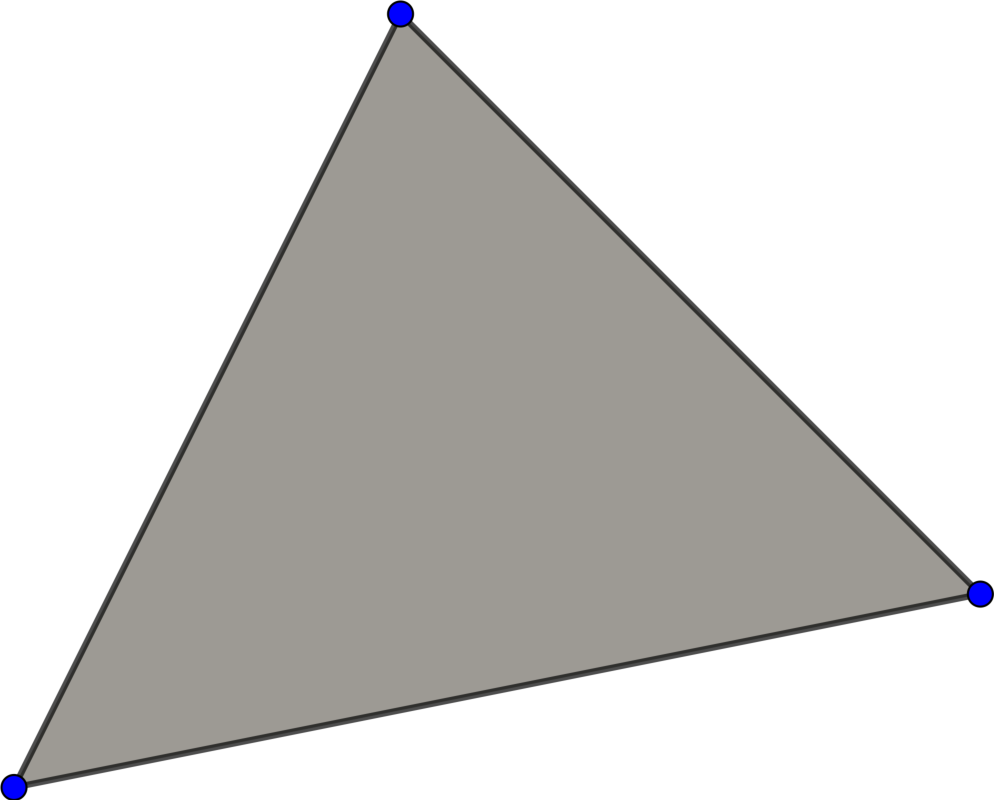
\includegraphics[scale=0.25]{images/P1.pdf}}   & \multirow{2}{*}{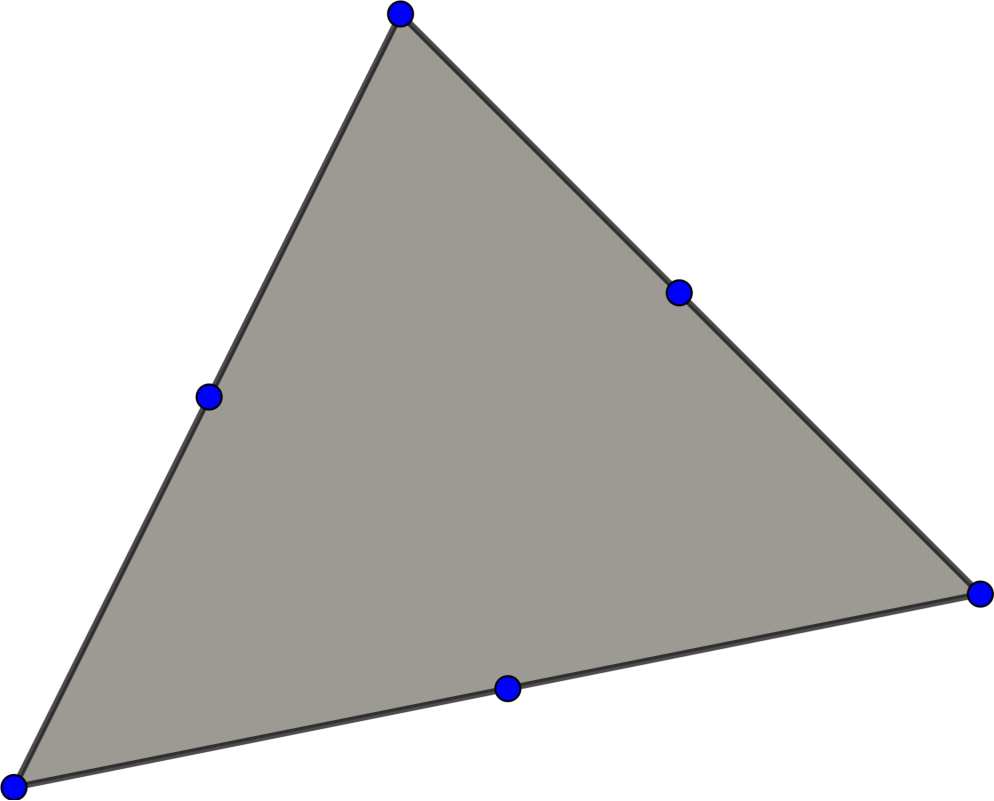
\includegraphics[scale=0.25]{images/P2.pdf}}   & \multirow{2}{*}{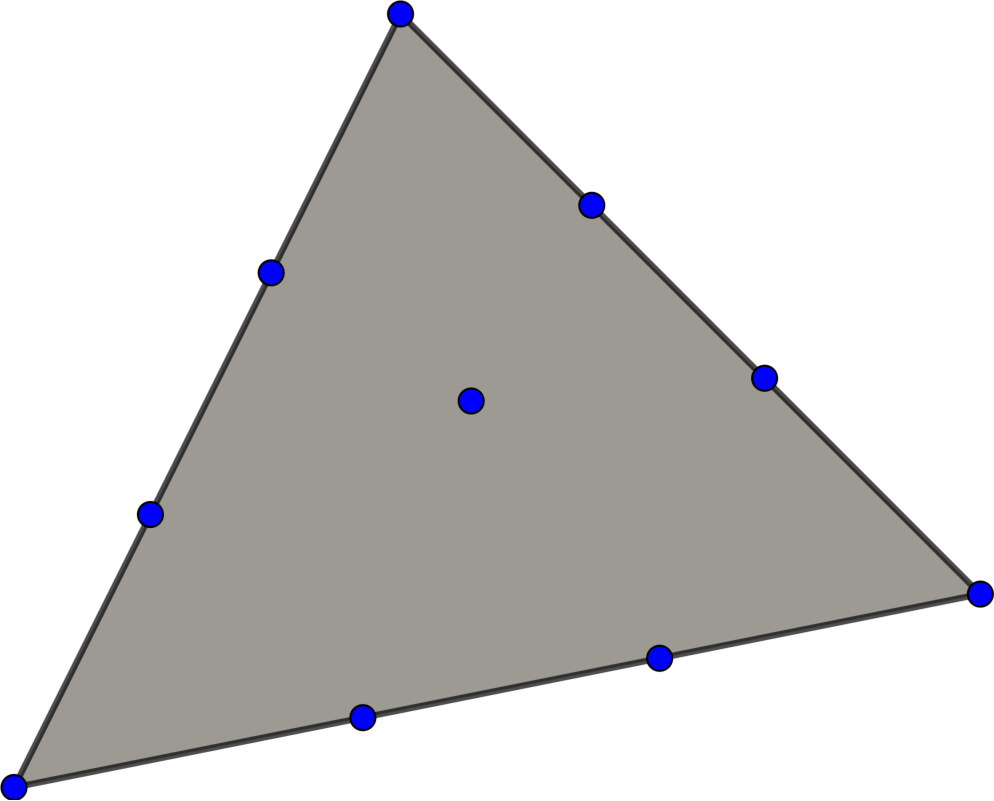
\includegraphics[scale=0.25]{images/P3.pdf}}   \\
&                          &                            \\
&&\\
&&\\
&&\\
&&\\
&&\\
&&\\
&&\\
\hline
\multirow{2}{*}{$\mathbb{Q}_1$} & \multirow{2}{*}{$\mathbb{Q}_2$}   & \multirow{2}{*}{$\mathbb{Q}_3$} \\
&&\\
\hline
&&\\
&&\\
\multirow{2}{*}{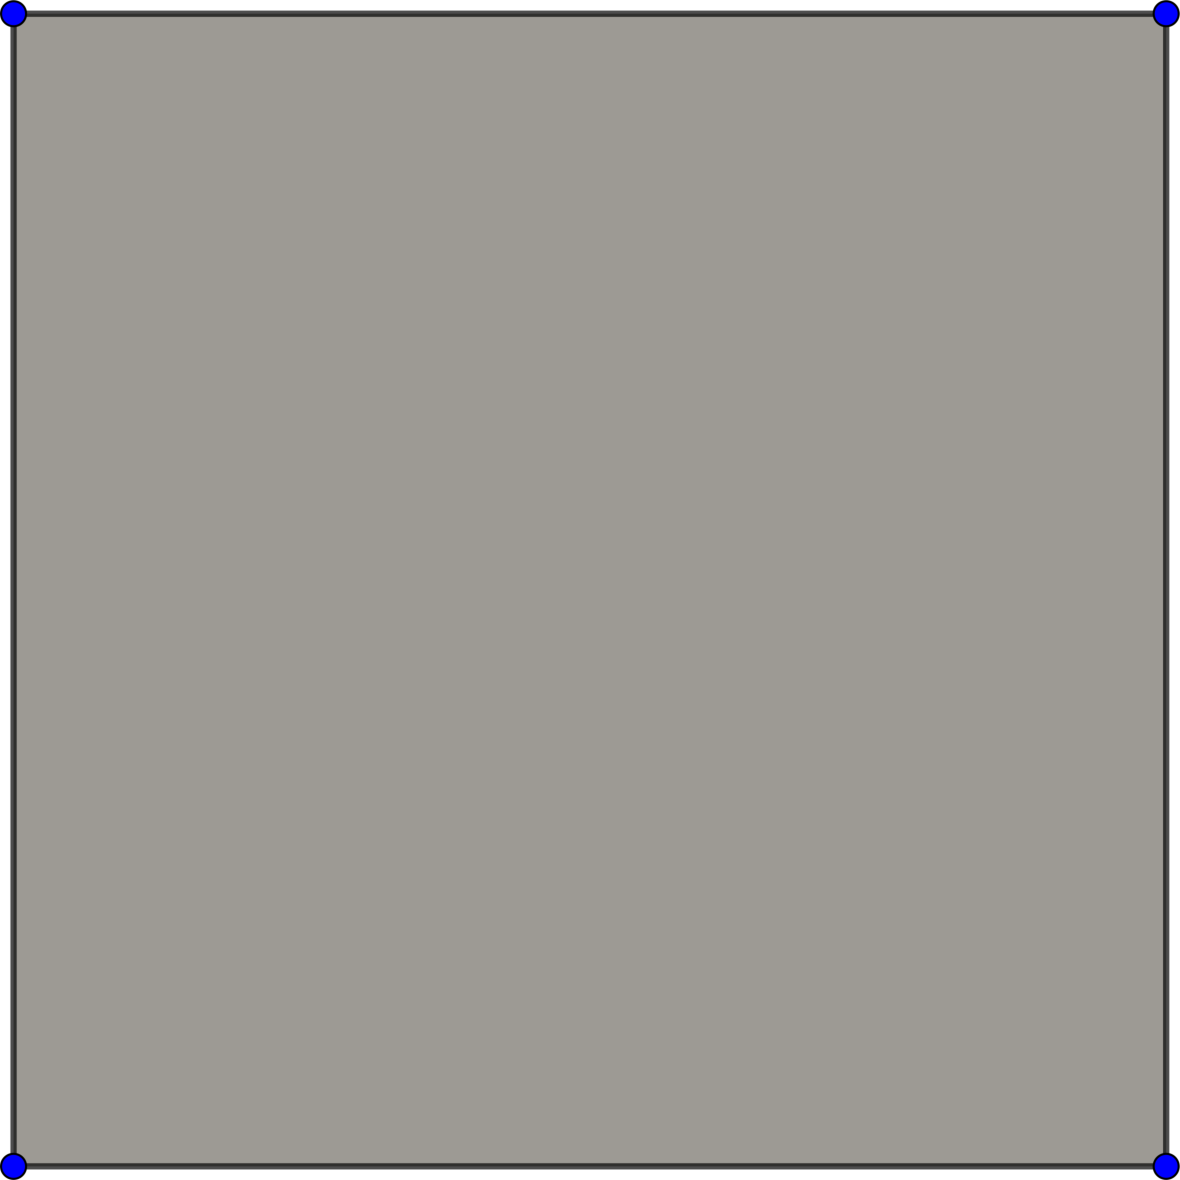
\includegraphics[scale=0.2]{images/Q1.pdf}}   & \multirow{2}{*}{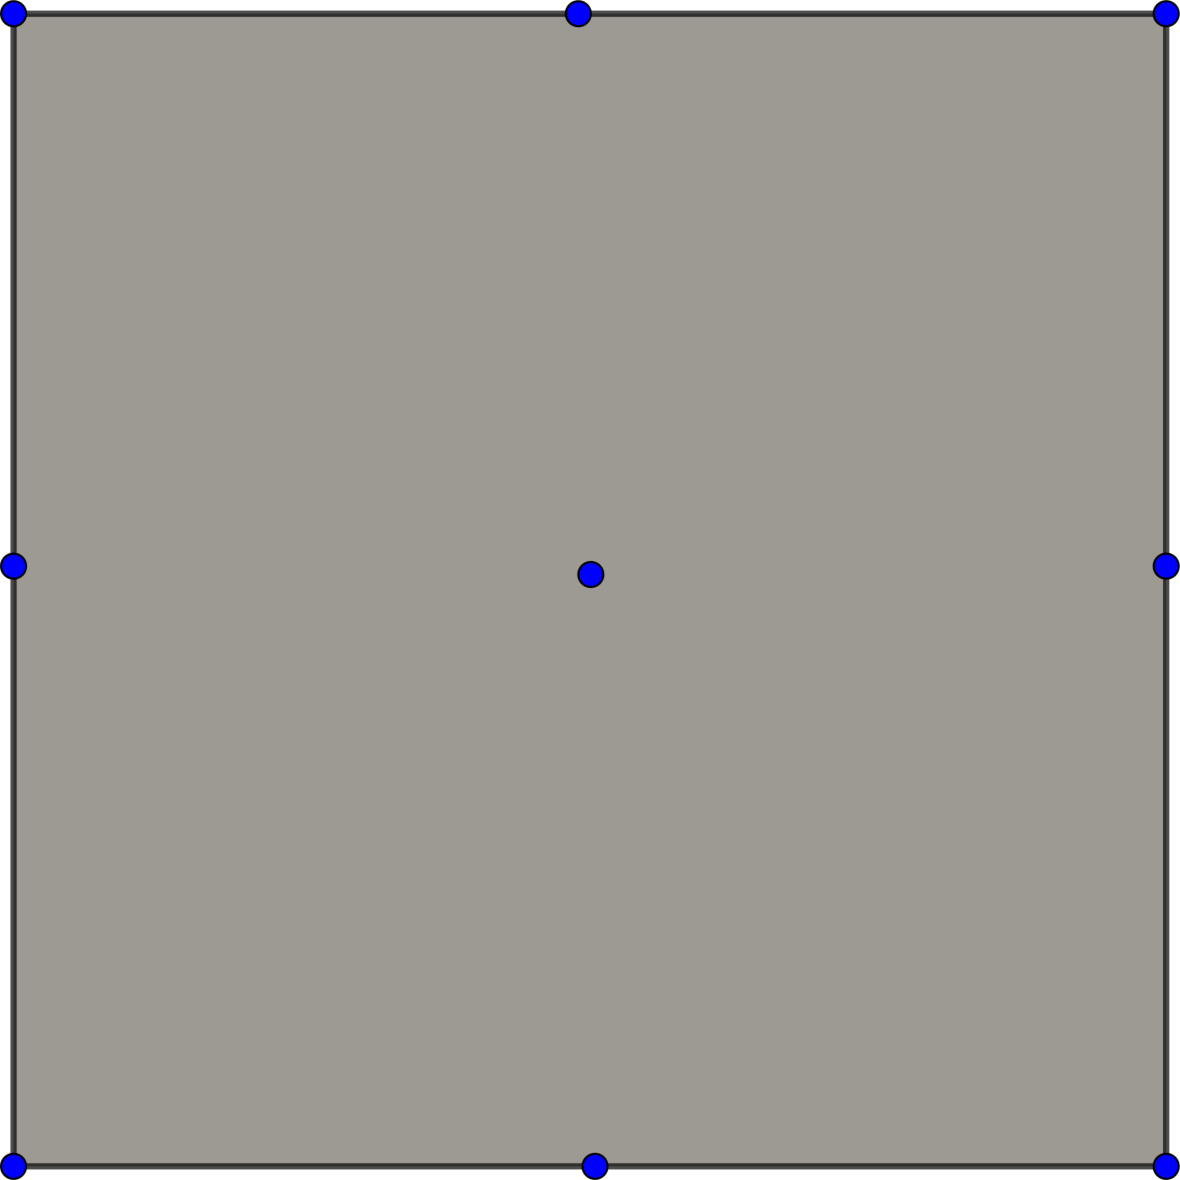
\includegraphics[scale=0.2]{images/Q2.pdf}}   & \multirow{2}{*}{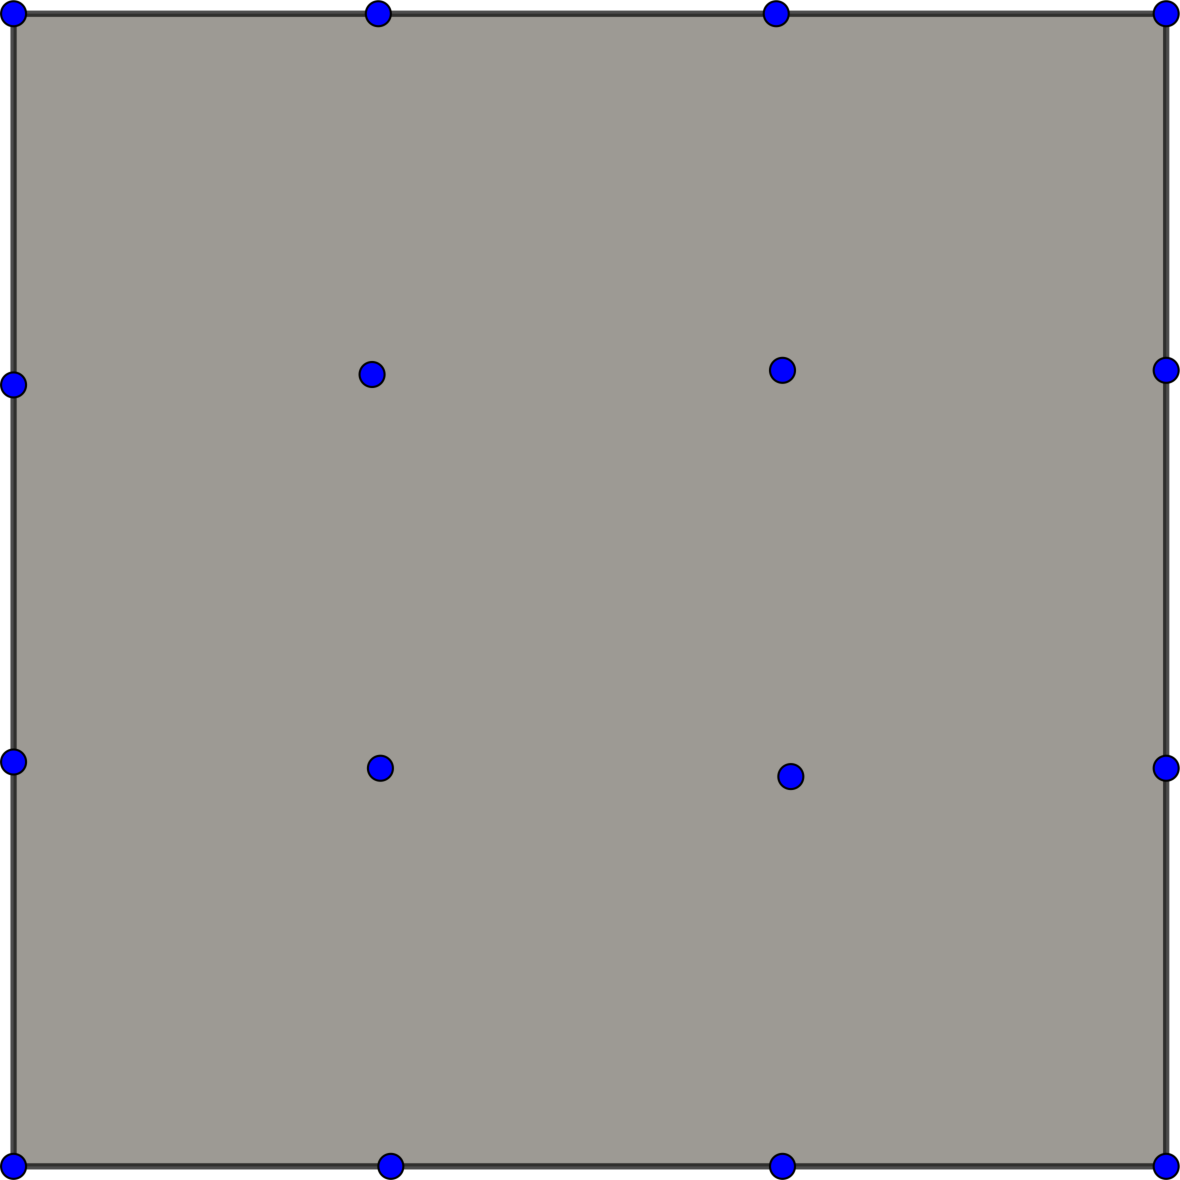
\includegraphics[scale=0.2]{images/Q3.pdf}}   \\
&&\\
&&\\
&&\\
&&\\
&&\\
&&\\
&&\\
&&\\
&&\\
&&\\
\hline
\end{tabular}
\caption{Illustration des degrés de liberté sur les éléments $\mathbb{P}_k$ et $\mathbb{Q}_k$ avec $k\in\{1,2, 3\}$.}
\label{tab:p1_vs_p2}
\end{table}

\begin{figure}[!h]
    \centering
    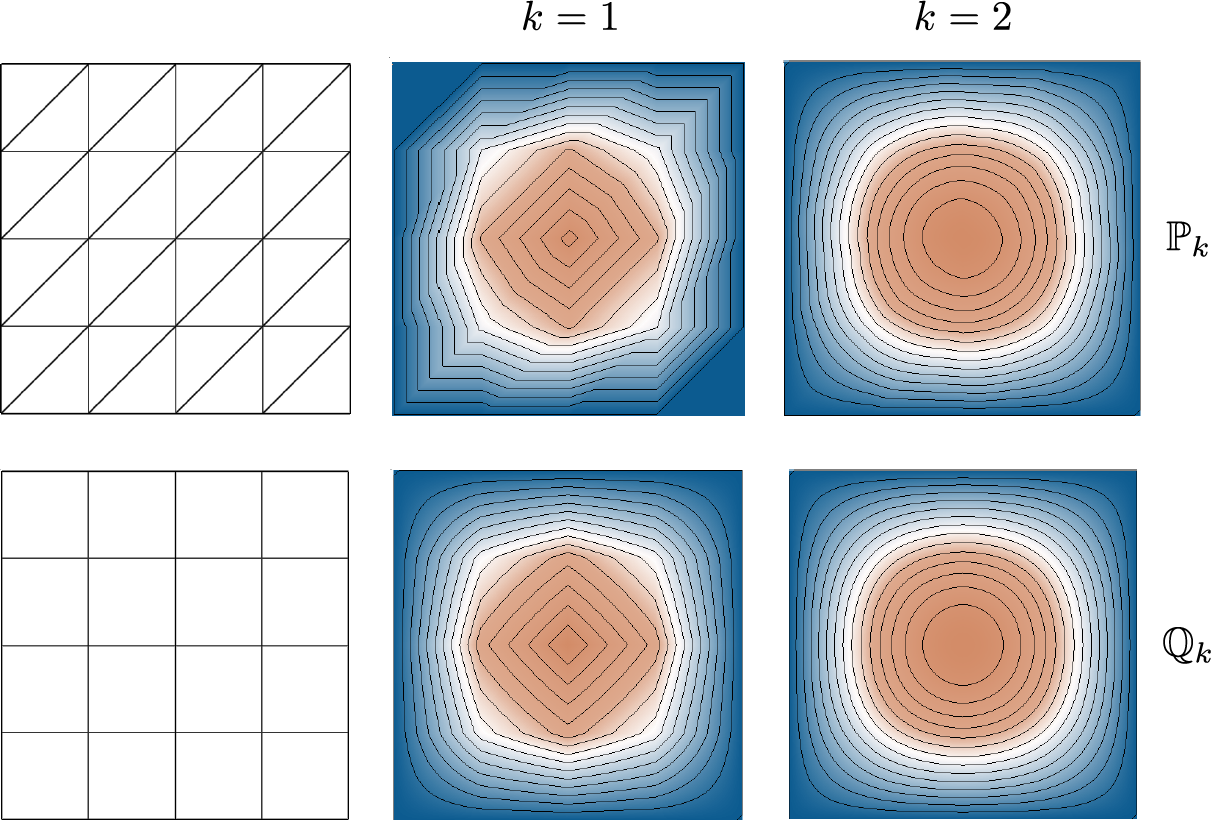
\includegraphics[scale=0.5]{images/comparaison_P_1_P_2.png}
    \caption{Solutions éléments finis de $-\triangle u=2\pi^2sin(\pi x)sin(\pi y)$ dans $\Omega$, $u=0$ sur $\partial\Omega$. Gauche: Maillage triangulaire et quadrilatéral. Milieu: Éléments d’ordre un. Droite: Éléments d’ordre deux. Source : \cite{reberol2018maillages}}.
    \label{fig:p1_vs_p2}
\end{figure}

Ainsi, les éléments $\mathbb{Q}_k$ sur quadrangle se révèlent être un choix optimal pour aborder des problèmes exigeant une précision extrême, tels que les simulations de déformations, la modélisation géométrique avancée et l'interpolation de formes complexes. Dans des domaines fortement élastiques et plastiques, les triangles linéaires sont notoirement reconnus pour leurs performances médiocres, car le maillage ne se déforme pas autant qu'il devrait. En revanche, les quadrilatères, comme mentionné dans \cite{shepherd2008hexahedral}, permettent de réduire à la fois l'erreur d'approximation et le nombre d'éléments par rapport aux triangles. Il est également intéressant de noter que les maillages quadrilatéraux ont besoin de moins d’éléments que les maillages triangulaires pour couvrir la même surface. Ces diférences se révèlent significatives pour des méthodes comme la méthode de Galerkin discontinue où il faut calculer des flux entre éléments, ou encore les méthodes d’hybridation \cite{reberol2018maillages}.

 Lors de la modélisation des ondes électromagnétiques par exemple, il est essentiel de prendre en compte les propriétés de continuité et de compatibilité des composantes tangentielles et normales des champs. Les éléments quadrangulaires offrent une base solide pour satisfaire à ces exigences car leurs arêtes et faces partagées permettent un alignement naturel des composantes. En conséquence, il est généralement plus simple et plus efficace de définir des fonctions de base qui préservent les propriétés de continuité et de compatibilité sur ces types de maillages. Cela se traduit par une formulation discrète plus directe des équations de Maxwell, où les termes de sauts et de sauts normaux entre les éléments adjacents peuvent être calculés plus facilement. De plus, les interpolations des champs électromagnétiques aux nœuds du maillage sont plus cohérentes, ce qui peut conduire à des résultats numériques plus précis et stables.

\subsubsection{Etirement anisotropique}

L'étirement anisotropique permet de contrôler la déformation d'un maillage d'une manière plus ciblée. Dans certaines situations, il est nécessaire de préserver la forme dans certaines directions tout en autorisant des déformations plus importantes dans d'autres directions. Selon la théorie de l'approximation, pour une surface donnée et une allocation de points déterminée, la manière la plus optimale d'obtenir une approximation de qualité est d'utiliser un maillage où les éléments sont agencés de manière rapprochée le long des directions principales de courbure \cite{d2000bilinear}. Par exemple, dans la modélisation de tissus biologiques ou de matériaux déformables, un étirement anisotropique peut permettre de simuler avec précision les caractéristiques de déformation du matériau. En mécanique des fluides, particulièrement pour les fluides visqueux, il est très important de modéliser avec un maillage très raffiné le comportement du fluide au contact d’un obstacle, car des variations très fortes des champs ont lieu dans cette couche limite \cite{reberol2018maillages}. De même, il est souhaitable de comprimer les éléments dans la direction normale de l'aile d'un avion car les phénomènes physiques les plus significatifs se produisent dans la couche limite \cite{bommes2013quad}.

Du fait que la couche limite tend généralement à être localement plane, avec une concentration notable dans la direction perpendiculaire à la surface, l'utilisation de maillages structurés se révèle particulièrement appropriée pour son modélisme. Cette pertinence est renforcée par la caractéristique des hexaèdres qui peuvent présenter une grande anisotropie tout en préservant des angles droits. 


Cependant, les maillages triangulaires peuvent être modifiés localement, ce qui leur permet de s’adapter plus facilement aux particularités des solutions.
Pour la mécanique, les quadrilatères/hexaèdres semblent plus intéressants, car ceux d'ordre 2 peuvent être modifiés afin d’atteindre des performances équivalentes aux tétraèdres quadratiques tout en conservant un coût de calcul bien inférieur.
Pour la propagation d’ondes électromagnétiques, l'optimisation des calculs numériques semble plus simple et efficace pour les éléments quadrilatéraux/hexaédriques qui ont naturellement une structure tensorielle.


%De plus, un certain nombre de modifications spécifiques à certaines applications (par ex. mécanique), comme l’utilisation de quadratures réduites ou de modes de déplacement incompatibles, sont couramment mises en oeuvre pour les quadrilatères et hexaèdres dans les logiciels commerciaux. Optimisation calculatoire de l’assemblage. Le calcul des coefficients (intégrales) repose sur des quadratures, c’est-à-dire des sommes pondérées. Lorsque les fonctions à intégrer sont des produits de polynômes uni-variés, comme c’est le cas pour Qk, il est possible de réduire le nombre d’opérations en factorisant des termes communs. Cette technique, dite de somme-factorisation, est particulièrement utile pour les polynômes d’ordres élevés et est une des raisons pour laquelle les maillages hexaédriques sont appréciés. Cette structure tensorielle rend également plus facile le développement de solveurs sans matrices, où les coefficients du système sont calculés à la volée lors de la résolution. Maillages structurés par blocs. Les maillages tétraédriques sont fondamentalement non structurés (par ex. valence des sommets très variable), il faut stocker toutes les informations de connectivité. Les maillages hexaédriques ont naturellement plus de régularité. Les maillages hexaédriques structurés sont combinatoirement équivalents à des grilles régulières. Dans ce cas, de nombreuses optimisations de calcul sont possibles, par exemple on peut connaitre à l’avance la largeur de bande des matrices creuses. Pour des géométries complexes, il n’est souvent pas possible d’utiliser des maillages globalement structurés, mais il est parfois possible de se ramener à des maillages structurés par blocs, pour lesquels ces optimisations peuvent être appliquées par bloc. Cette remarque ne s’applique pas à tous les maillages hexaédriques, mais la sous-catégorie des maillages structurés (par blocs) est très intéressante pour des applications hautes performances. Raffinement local. Comme les maillages hexaédriques sont plus ou moins structurés, il n’est généralement pas possible de leur appliquer des opérations de raffinement locales et de conserver un maillage conforme. Raffiner un hexaèdre engendre des modifications qui se propagent à travers une grande partie du modèle. Sur ce point, les maillages tétraédriques sont beaucoup plus flexibles, il existe d’ailleurs de nombreuses techniques de raffinement adaptatif pour ces derniers. Le raffinement adaptatif est particulièrement intéressant dans le cadre de la méthode des éléments finis puisqu’il 23 1.4. Variantes offre la possibilité d’augmenter la précision de la solution approchée tout en impactant peu le temps de calcul. Cette approche est parfois appelée h-FEM, car h caractérise la taille des éléments, en opposition à l’approche p-FEM où la précision de la solution est améliorée en augmentant le degré des polynômes d’interpolation. Les méthodes hp-FEM combinent ces deux outils. Nombre d’éléments et nombre de faces.  Maillages hex-dominants : generation, simulation et evaluation THESE presentee et soutenue publiquement le 23 mars 2018 pour l'obtention du Doctorat de l'Universite de Lorraine (mention informatique) par Maxence Reberol

 \subsubsection{Intégration numérique}

 Les méthodes de quadrature sont fréquemment utilisées dans le contexte de la simulation numérique pour calculer des quantités telles que l'aire d'un quadrilatère déformé, le moment d'inertie, ou d'autres intégrales associées à des propriétés physiques. Ces quantités nécessitent souvent l'intégration de fonctions sur les éléments (triangles, quadrilatères) déformés. Les méthodes de quadrature adaptées à la géométrie et à la structure tensorielle du quadrilatère permettent d'approximer ces intégrales de manière efficace et précise.
 
Lorsqu'on travaille avec des maillages triangulaires, les formules d'intégration numérique doivent prendre en compte les coordonnées barycentriques. Ces coordonnées sont utilisées pour représenter un point à l'intérieur d'un triangle en fonction de ses sommets. Cela peut rendre les formules d'intégration plus complexes à définir et à calculer. Les transformations entre les coordonnées réelles et barycentriques ainsi que les calculs associés peuvent ajouter une couche de complexité. En revanche, les maillages quadrangulaires ont des avantages en termes de simplicité. Puisque les éléments sont des quadrilatères, les coordonnées barycentriques ne sont pas nécessaires pour effectuer des calculs d'intégration. Les formules d'intégration sur des quadrilatères sont plus intuitives, car vous pouvez généralement utiliser des coordonnées cartésiennes standard pour décrire les points à l'intérieur de chaque élément. Cela simplifie grandement les calculs et les rend plus compréhensibles.

Les quadrilatères peuvent être plus facilement paramétrés en utilisant des coordonnées locales qui varient de 0 à 1 dans les deux directions principales. Cette paramétrisation facilite la définition des fonctions d'intégration et réduit la complexité des transformations géométriques et les calculs de jacobienne.\\


Toutefois, si la génération de maillages simplextiques (triangles) est très développée depuis plus d'un demi-siècle, celle de quadrilatères ou d'hexaèdres est plus problématique.
Dans le cas du maillage triangulaires, des algorithmes sont disponibles même pour des géométries très complexe. Cependant, les algorithmes de génération de maillage quadrilatéral automatisé sont disponibles pour une classe de géométries très limitée. Malgré les avancées dans la génération de maillages automatisés, la création de maillages de haute qualité reste un défi dans de nombreux cas, en particulier pour les géométries complexes. De ce fait, la génération de maillages demeure un domaine de recherche actif et important \cite{shepherd2008hexahedral}.

\section{Maillage}

Un maillage est une discrétisation d'un espace ou d'un domaine en cellules élémentaires (triangle ou rectangles en 2D, tétraèdres ou hexaèdres en 3D). De manière plus générale, un assemblage d’éléments, est considéré comme un maillage si \cite{george2013mesh}:\\

\begin{itemize}
\item l’union des éléments est une approximation de l’objet ou du domaine,\\
\item l’intérieur de chaque élément n’est pas vide,\\
\item l’intersection de l’intérieur de deux éléments est vide.\\
\end{itemize}

 Dans le contexte de la résolution des équations aux dérivées partielles en deux dimensions (2D), il existe différents types de maillages utilisés pour la discrétisation du domaine. Passons en revue quelques-uns de ces types de maillages couramment utilisés.

\subsection{Maillages à bases de triangles}


Il y a diverses approches pour créer des maillages en utilisant des triangles. On peut les regrouper en trois grandes catégories : les méthodes de type Delaunay, les méthodes basées sur des fronts et les méthodes de découpe spatiale, comme évoqué dans la référence \cite{botella2016generation}.

\subsubsection{Méthode de Delaunay}
Les méthodes de type Delauney se basent sur le critère de Delauney. Ce critère parfois appelé "propriété de la boule vide", stipule pour tout triangle, aucun sommet ne doit être contenu dans la boule ouverte correspondant au cercle circonscrit au triangle.

Bien que le critère de Delaunay soit connu depuis de nombreuses années, ce n'est que grâce aux travaux de Charles Lawson et Dave Watson que le critère a été largement popularisé et utilisé dans les méthodes de maillage \cite{owen1998survey}. La règle de Delaunay, en soi, ne constitue pas un algorithme pour générer des maillages. Elle représente plutôt un critère qui guide la manière de connecter un ensemble de points préexistants dans l'espace. Pour mettre en place un maillage, il est nécessaire de définir les emplacements des nœuds à l'intérieur de la géométrie. Une approche courante consiste d'abord à mailler la frontière de la géométrie, créant ainsi un ensemble initial de nœuds. Ensuite, les nœuds le long de cette frontière sont connectés pour former des triangles qui respectent la règle de Delaunay. À mesure que de nouveaux nœuds sont insérés itérativement dans le maillage existant, les triangles ou tétraèdres à une échelle locale sont ajustés pour maintenir en permanence la conformité à la règle de Delaunay. Ce qui distingue une méthode de génération de maillage de type Delaunay d'une autre, ce sont les algorithmes spécifiques utilisés pour déterminer les positions des nœuds à l'intérieur de la géométrie.\cite{owen1998survey}.

\paragraph{Maillage de Delauney-Voronoï}
Dans ce processus, on détermine la disposition géométriquement optimale d'un ensemble de sommets. Pour y parvenir, on réalise un échantillonnage du modèle en plaçant les points de manière aléatoire ou en suivant une heuristique spécifique. Ensuite, la position géométrique de ces points est affinée en minimisant une fonction objectif qui reflète une distribution idéale prédéfinie \cite{botella2016generation}. Ensuite, les diagrammes de Voronoï de ces points sont générés :

\begin{definition}[\cite{hecht2007maillage}, voir figure \ref{fig:voronoi_diagram}]
Soit un ensemble de points $\mathcal{S}=\{x^i\in\mathbb{R}^2, i\in\llbracket 1, N_p\rrbracket\}$. Les diagrammes de Voronoï sont les polygones convexes $V^i$, pour $i\in\llbracket 1, N_p\rrbracket$, formés par l’ensemble des points de $\mathbb{R}^2$ qui sont plus proches de $x^i$ que des autres points $x^j$. Formellement, on a:
\begin{eqnarray}
V^i=\{x\in\mathbb{R}^2\ |\ |x-x^i|\leq|x-x^j|,\ \forall j\in\llbracket 1, N_p\rrbracket\}.
\end{eqnarray}
\end{definition}

\begin{figure}[!h]
    \centering
    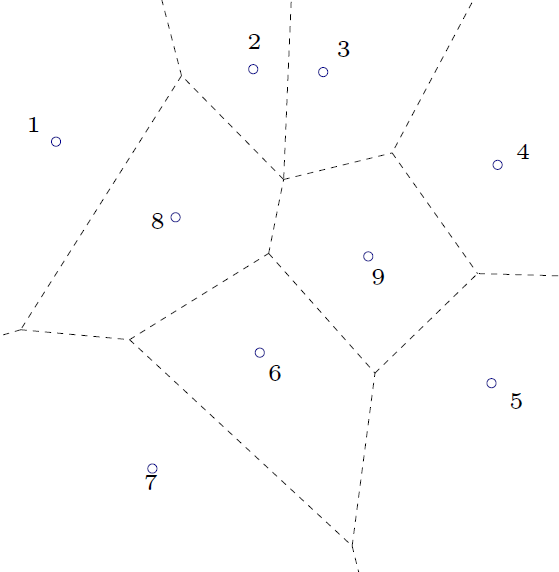
\includegraphics[scale=0.6]{images/voronoi_diagram.png}
    \caption{Diagramme de Voronoï. Source : \cite{hecht2007maillage}.}
    \label{fig:voronoi_diagram}
\end{figure}

Le maillage de Delaunay est ensuite généré en tant que maillage dual des diagrammes de Voronoï. Deux points $x_i$ et $x_j$ sont reliés dans ce maillage si les diagrammes de Voronoï $V_i$ et $V_j$ partagent un segment en commun (voir figure \ref{fig:maillage_delauney}). Afin d'obtenir un maillage triangulaire, il suffit de diviser les polygones qui ne sont pas déjà des triangles en triangles.

\begin{figure}[!h]
    \centering
    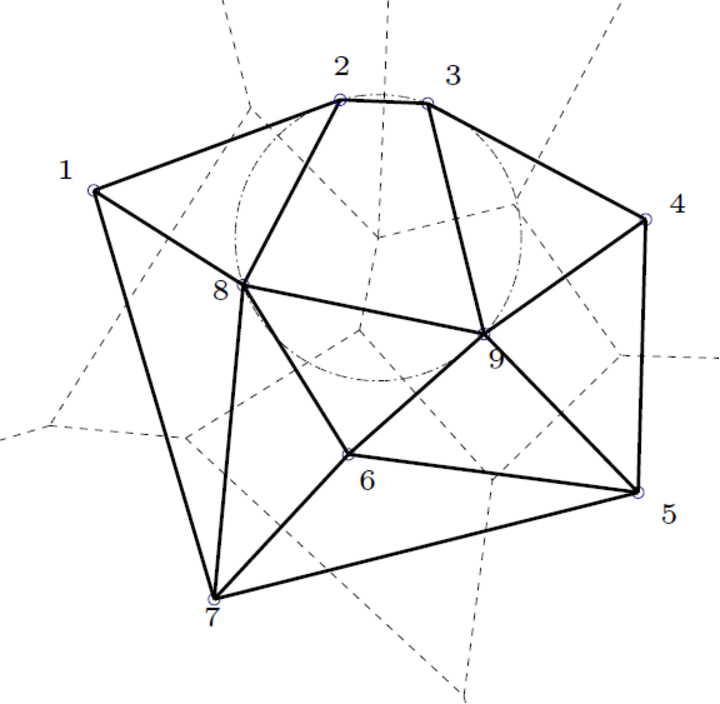
\includegraphics[scale=0.65]{images/Maillage_delauney.pdf}
    \caption{Maillage de Delauney. Source : \cite{hecht2007maillage}.}
    \label{fig:maillage_delauney}
\end{figure}

\paragraph{L'algorithme de Bowyer-Watson} construit les triangulations de Delaunay par induction \cite{bowyer1981computing, watson1981computing, ern2004theory}.
 est une méthode de triangulation de Delaunay en 2D. Son objectif est de générer un maillage de triangles de Delaunay pour un ensemble de points donné dans le plan. L'algorithme commence par créer un triangle géant qui englobe tous les points de l'ensemble. Ensuite, il ajoute chaque point un par un dans le maillage en respectant la règle de Delaunay, c'est-à-dire que le cercle circonscrit de chaque triangle du maillage doit être vide, ne contenant aucun autre point de l'ensemble. Pour ajouter un point dans le maillage, l'algorithme identifie tous les triangles du maillage qui sont affectés par l'ajout du nouveau point. Il supprime ces triangles du maillage et forme de nouveaux triangles avec le point ajouté comme sommet. Le processus se répète jusqu'à ce que tous les points soient ajoutés et que le maillage respecte la propriété de Delaunay.

Les méthodes de type Delaunay ne fournissent pas de garantie pour préserver la discrétisation des frontières du modèle. Deux stratégies sont mises en œuvre pour assurer que la discrétisation des limites soit préservée dans la triangulation de Delaunay \cite{botella2016generation}:\\

\begin{itemize}
    \item L'ajout de sommets le long des frontières jusqu'à ce qu'elles correspondent géométriquement. Cependant, cela peut altérer la discrétisation initiale \cite{cohen2002conforming}.\\
    \item Effectuer des modifications locales sur le maillage pour obtenir la discrétisation initiale des frontières. Une description détaillée de ce processus est donnée dans les ouvrages de George et Borouchaki \cite{george1997triangulation} ainsi que de Hecht \cite{hecht2007maillage}.
    
    Considérons que l'arête $(\alpha, \beta)$ ne fait pas partie du maillage de Delaunay. Nous analysons les diagonales $(a, c)$ des quadrilatères $(a, b, c, d)$ convexes constitués de deux triangles $(a, b, c)$ et $(b, c, d)$ où la diagonale $(a, c)$ coupe $(\alpha, \beta)$. Si l'arête $(b, d)$ ne coupe pas $(\alpha, \beta)$, nous procédons à l'échange de diagonales. Dans le cas contraire, l'échange de diagonales est effectué de manière aléatoire. Du fait qu'il existe une solution au problème, le recours aux échanges de diagonales de manière aléatoire permet de converger, car, statistiquement, tous les maillages possibles sont parcourus et ils sont en nombre fini.
\end{itemize}


\subsubsection{Méthode frontale}

La méthode d'avancée de front \cite{george1994advancing, lohner1996progress, lohner2014recent} se distingue par son approche qui débute avec une frontière préalablement définie constituée d'un ensemble d'arêtes qui reste inchangée tout au long du processus de génération du maillage. Cette frontière triangulée est considérée comme le front à partir duquel de nouveaux éléments sont progressivement ajoutés.

À chaque itération, il est décidé où positionner le prochain sommet du front. Cette décision est généralement prise en recherchant la position la plus appropriée sur la frontière, dans le but de réduire les déformations des triangles et d'assurer une qualité élevée du maillage. Cependant, dans certaines situations particulières, on peut préférer d'autres critères en fonction des besoins spécifiques de l'application. Par exemple :\\

\begin{itemize}
    \item Critère de Delaunay : le sommet est sélectionné de manière à respecter le critère de Delaunay, ce qui implique que le cercle circonscrit au nouveau triangle formé ne doit pas englober d'autres points de la géométrie.\\
    \item Critère de qualité de l'élément: pour garantir que tous les triangles du maillage ont des angles proches de 60 degrés ou satisfont d'autres propriétés de forme souhaitées\\
    \item Critère de densité: pour contrôler la taille des éléments dans différentes régions du domaine. Par exemple, on peut souhaiter avoir des éléments plus petits dans les régions où des variations importantes du champ numérique sont attendues\\
\end{itemize}


Les bords des triangles initiaux du front deviennent alors des faces intérieures du maillage, tandis qu'un nouveau jeu de faces de front est créé. Ce cycle continue jusqu'à ce que le maillage couvre entièrement le domaine. Ainsi, cette approche assure une discrétisation cohérente du domaine en suivant rigoureusement la frontière prescrite, et ce, de manière incrémentale \cite{baker2005mesh}.

Au fur et à mesure de l'avancement du front, il devient possible d'enrichir la qualité du maillage en procédant à des opérations de raffinement. Ces opérations englobent l'insertion de points au milieu des arêtes ainsi que l'ajustement des positions des sommets, permettant ainsi une meilleure adaptation aux courbes présentes sur la surface. Il est également envisageable de prendre en considération d'autres contraintes particulières, telles que les conditions aux limites, ou encore des critères spécifiques de qualité de maillage au sein de zones spécifiques de l'objet.

Une difficulté particulière avec cette méthode survient dans les étapes finales lorsque le front se réduit progressivement et les derniers espaces vides sont remplis par de nouveaux éléments. Cela est illustré sur la figure \ref{fig:moving_front_method}, où l'on peut voir une triangulation presque achevée de la région autour d'un profil d'aile, avec les arêtes du front actuel marquées en gras.  Une étape d'optimisation peut alors être requis pour une disposition optimale des sommets \cite{botella2016generation}.

\begin{figure}[!h]
    \centering
    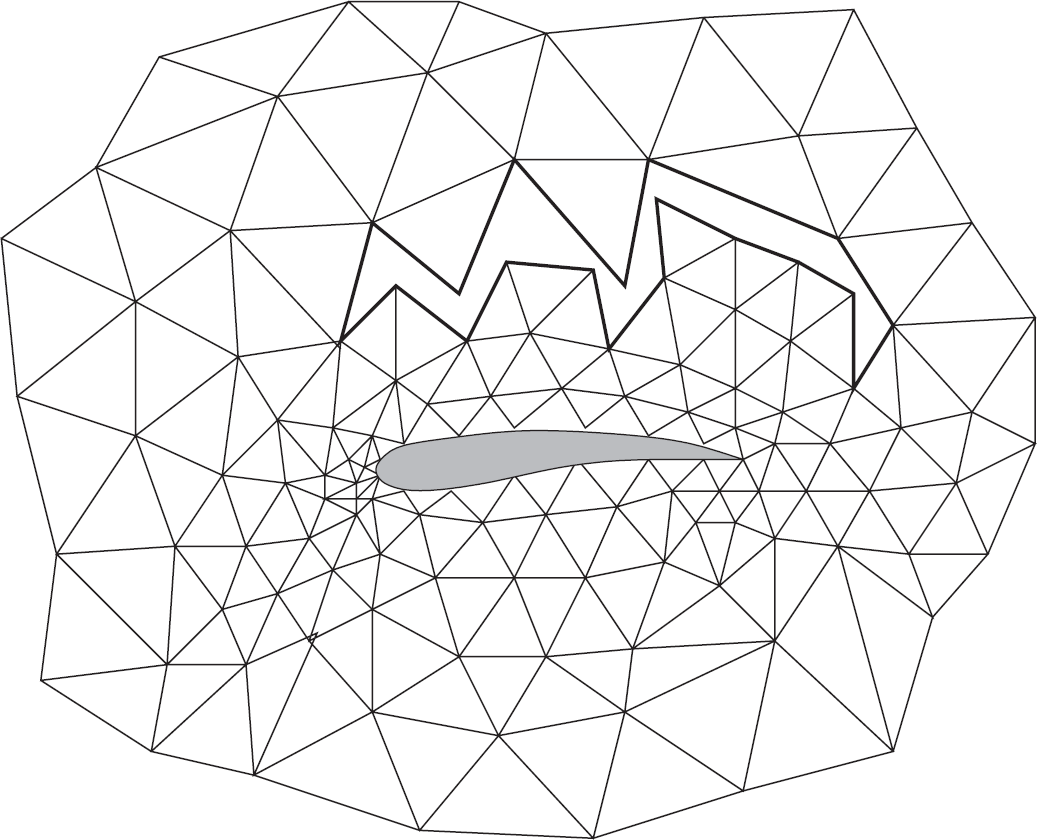
\includegraphics[scale=0.4]{images/moving front method.png}
    \caption{Phase de fermeture de la méthode du frontale. Source : \cite{baker2005mesh}.}
    \label{fig:moving_front_method}
\end{figure}


La méthode d'avancée de front est relativement aisée à implémenter et peut être efficace pour des géométries simples ou modérément complexes. Cependant, pour des géométries très complexes ou avec des trous, il peut être difficile de construire une frontière active appropriée, et le maillage résultant peut contenir des triangles de mauvaise qualité.

Il existe différentes variantes de la méthode d'avancée de front qui peuvent être adaptées en fonction des caractéristiques de la géométrie à mailler et des exigences du problème. Des améliorations peuvent être apportées pour contrôler la qualité des triangles, optimiser la distribution des points, gérer les singularités ou les contours concaves, etc. En général, la méthode d'avancée de front est un outil polyvalent et largement utilisé pour la génération de maillages triangulaires dans de nombreuses applications scientifiques et d'ingénierie.

\subsubsection{Méthode de décomposition spatiale (Quadtree)}

Introduite par  \cite{yerry1983finite}, cette procédure peut être vue comme une division du domaine en une collection de rectangles, suivie d'une division de ces rectangles en triangles \cite{baker2005mesh}.

Ces méthodes se basent sur une structure d'arbre qui est une représentation hiérarchique des différentes subdivisions de l'espace. Schématiquement, l'approche de maillage basée sur les quadtrees se compose des étapes suivantes:

%de trois étapes successives et peut être résumée comme suit  Un premier rectangle est formé, qui contient tous les points du contour. La méthode consiste à découper, à partir de ce rectangle initial, chaque rectangle en 4 rectangle, de façon récursive, tant que les limites du modèle intersectent la cellule, jusqu’à un critère d’arrêt . Ce critère d’arrêt peut être conditionné par la taille d’éléments locale souhaitée, par la courbure du modèle présent dans la cellule, ou un nombre de subdivisions. Un autre critère, permettant de conserver la topologie du modèle, est de minimiser le nombre de composantes connexes de l’intersection entre le modèle et une cellule \cite{botella2016generation}. Schématiquement, l'approche de maillage basée sur les quadtrees se compose de trois étapes successives et peut être résumée comme suit \cite{pascal1998fast}:\\

\begin{enumerate}
    \item Initialisation : on commence par définir le domaine global à mailler puis on crée un quadrilatère initial qui le représente.
    
    \item Subdivision du quadtree : le quadrilatère initial est divisé en quatre sous-quadrants de taille égale en traçant deux lignes verticales et deux lignes horizontales pour former une grille.
    
    \item Évaluation des critères : pour chaque sous-quadrant nouvellement créé, on évalue des critères de qualité de maillage tels que la taille des angles, la longueur des arêtes et d'autres mesures géométriques pour déterminer s'il est nécessaire de subdiviser davantage ou si le sous-quadrant est adéquat pour la triangulation.
    
    \item Triangulation des sous-quadrants : les sous-quadrants jugés appropriés pour la triangulation sont convertis en triangles en reliant leurs coins.
    
    \item Raffinement : si nécessaire, on effectue des opérations de raffinement, telles que l'ajout de points au milieu des arêtes ou l'ajustement des sommets pour mieux s'adapter aux caractéristiques de la surface.
    
    \item Itérations : répétez les étapes 3 à 5 pour les sous-quadrants nouvellement créés, en continuant à subdiviser et à trianguler jusqu'à ce que les critères de qualité de maillage soient satisfaits dans toutes les zones du maillage.
    
    \item Terminaison : on arrête le processus de subdivision et de triangulation lorsque les critères de qualité de maillage sont globalement atteints ou lorsque d'autres conditions de terminaison spécifiques sont satisfaites.
    
    \item Fin : le processus se termine avec un maillage triangulaire satisfaisant les critères de qualité établis pour la région donnée.
\end{enumerate}

Afin de ne pas avoir de trop grandes variations de taille d’éléments dans le maillage, la différence de niveaux de subdivision entre deux cellules adjacentes est limitée. Une fois la décomposition terminée, les sommets du maillage sont les coins des cellules de subdivisions et éventuellement les intersections entre les limites du modèle et les cellules. Les éléments du maillage sont alors construits en découpant les cellules \cite{botella2016generation}.


\begin{figure}[!h]
    \centering
    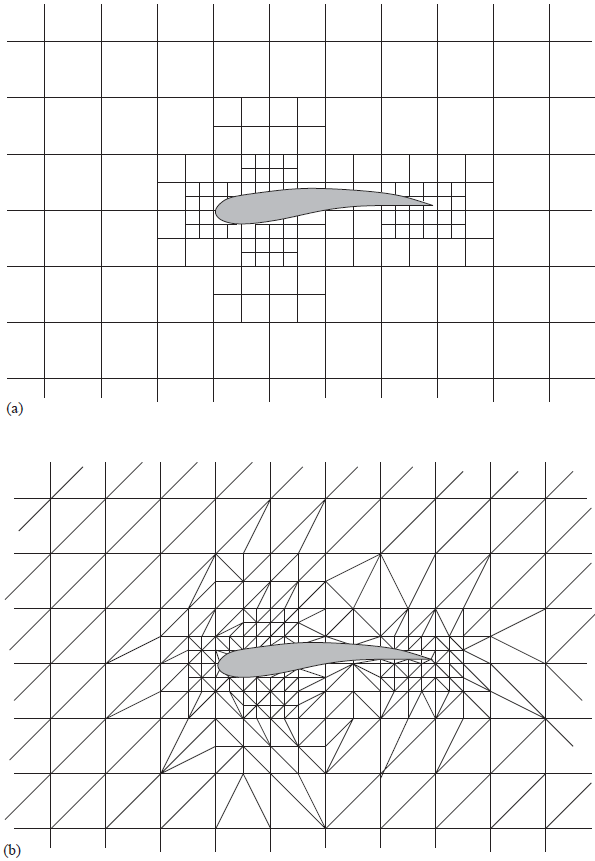
\includegraphics[scale=0.65]{images/octree decomposition.png}
    \caption{(a) Décomposition en octree de la région autour d'un profil aérodynamique. (b) Conversion de la décomposition en octree en une triangulation. Source : \cite{baker2005mesh}}
    \label{fig:octree decomposition}
\end{figure}

La méthode Quadtree permet de concentrer les ressources de maillage dans les zones les plus complexes ou les plus intéressantes, tout en conservant des éléments de maillage plus simples dans les régions homogènes. Cela conduit à une utilisation efficace des ressources de calcul et de stockage. Elle permet d'obtenir des maillages de haute résolution là où c'est nécessaire, tout en réduisant la complexité dans les zones moins critiques. Par ailleurs, elle gère efficacement les discontinuités géométriques et topologiques en adaptant la taille et la forme des éléments de maillage autour de ces régions, ce qui améliore la précision des simulations.

Cependant, la mise en œuvre de cette méthode nécessite des algorithmes sophistiqués pour gérer la subdivision récursive, la fusion de carrés et la gestion des bordures. Le choix des critères pour la subdivision et le raffinement des carrés peut être complexe et dépendant de l'application, ce qui nécessite une expertise dans le domaine concerné. Pour finir, l'adaptation du maillage près des frontières du domaine peut nécessiter une attention particulière pour éviter des problèmes de cohérence.

%Compte tenu de leur régularité, les maillages structurés sont géométriquement peu flexibles et le plus souvent constitués de quadrilatères. Ces maillages sont fréquemment appelés des grilles. En revanche, les maillages non structurés peuvent être composés de polygones quelconques, ce qui augmente leur capacité à représenter des géométries complexes. Si le maillage est composé de plusieurs types d’éléments différents, il est dit multi-éléments ou mixte \cite{ref7}.\\
%Lors des simulations numériques, le maillage se révèle indispensable puisqu'il est le support de méthodes numériques telles que les éléments finis, les volumes finis ou les différences finies. Il joue non seulement le rôle de partition du domaine, mais aussi de support pour les polynômes d'interpolation utilisés. Il permet notamment de générer des systèmes linéaires creux que l’on peut résoudre efficacement.\\
%Les simulations numériques requièrent donc la construction de "bons maillages". Ils doivent représenter suffisamment les géométries présentes dans la scène de calculs en fonction des physiques étudiées et posséder des éléments de "bonnes qualités" afin d'assurer de bonnes propriétés aux schémas numériques (précision, conditionnement du système linéaire). Ci-dessous, nous présentons quelques méthodes de construction de maillages.

\subsection{Maillages à bases de quadrilatères}

Les maillages à bases de quadrilatères sont caractérisé par la nature des sommets qui les composent. Un sommet dans un tel maillage est dit \emph{régulier} si sa \emph{valence} topologique est égale à 4; sinon il est dit \emph{irrégulier}. La valence topologique d'un sommet est le nombre de faces adjacentes à ce sommet. Avec cette propriété, les maillages quadrilatéraux peuvent être décrit en terme de régularité de la manière suivante \cite{bommes2013quad} (voir figure \ref{fig:Quad_meshes_categories}):\\

 \begin{itemize}
    \item Maillage non-structuré : une grande partie des sommets du maillages sont des sommets irréguliers,\\
    \item Maillage à valence semi-régulière : la plupart des sommets du maillage sont des sommets réguliers,\\
    \item Maillage semi-régulière : il s'agit d'un maillage formé de plusieurs partitions. Chaque partition est un réseau de quadrilatères de sommets réguliers, et l'ensemble est assemblé de manière \emph{conforme}, c'est-à-dire que les interfaces entre les partitions s'ajustent de manière cohérente,\\
    \item Maillage régulier :  il ne contient aucun sommet irrégulier. Un maillage régulier est topologiquement équivalent à une grille régulière.\\
 \end{itemize}
 
\begin{figure}[!h]
    \centering
    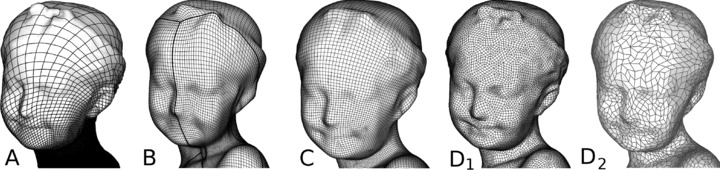
\includegraphics[scale=5.2]{images/Quad_meshes_categories.png}
    \caption{Catégories de maillage quadrilatéral. A: régulier; B: semi-régulier; C: valence semi-régulier; D1-D2: non-structuré (D2 plus irrégulier que D1). Source: \cite{bommes2013quad}.}
    \label{fig:Quad_meshes_categories}
\end{figure}


Dans le contexte des simulations numériques, les caractéristiques recherchées pour les maillages quadrilatéraux revêtent une importance significative. Les attributs visés se déclinent généralement comme suit :\\

\begin{itemize}
    \item Minimalité des irrégularités : il est préférable d'avoir le moins possible de points irréguliers dans les maillages puisque dans leur voisinnage, les mailles s'éloignent de la forme typique carré. La minimisation de ces irrégularités contribue donc à maintenir la cohérence et la régularité du maillage, améliorant ainsi la stabilité et la précision des simulations.\\
    \item Alignement le long de la frontière : il est souhaitable que les éléments du maillage soient alignés le long des bords du domaine permettant ainsi de donné une description fidèle du bord du domaine.\\
    \item Éléments de haute qualité : il est recommandé d'utiliser des éléments dont les contours se rapprochent au maximum de la configuration d'un carré ou d'un rectangle. En utilisant un maillage composé d'éléments qui présentent des formes régulières, on peut minimiser les risques de dégénérescence lors des transformations géométriques causées par des éléments déformés ou excessivement étirés.\\
    \item Respect des contraintes de taille : il est essentiel que les éléments du maillage satisfaissent aux exigences de taille définies. Cette condition garantit que le maillage capture de manière appropriée les variations locales de la solution, en allouant davantage de détails là où c'est nécessaire, tout en maintenant une efficacité numérique globale.\\
    \item Insensible à l'orientation. La rotation ou la translation d'une géométrie donnée ne devrait pas changer la topologie du maillage résultant. Un maillage généré dans une géométrie transformée devrait être équivalent au maillage original transformé.\\
\end{itemize}

Générer des maillages qui incorporent simultanément chacune de ces propriétés constitue un défi ardu. Très souvent, la poursuite de l'une de ces caractéristiques entre en conflit avec la quête d'optimisation d'une autre. Plusieurs approches ont été développées pour la génération de maillages quadriatères. Ces approches varient en fonction des besoins spécifiques des applications, de la complexité de la géométrie à mailler et des contraintes de qualité du maillage requis. 

\subsubsection{Décomposition de maillages triangulaires en quadrangles}

Les méthodes de conversion de maillages triangulaires en maillages quadrangulaires, également appelées \emph{méthodes de maillage tri-to-quad}, visent à transformer des maillages constitués de triangles en maillages contenant principalement des quadrilatères (quads).  Il existe plusieurs approches pour effectuer cette conversion, chacune ayant ses avantages et ses limitations. Voici quelques-unes des méthodes couramment utilisées :

Sous-division de Catmull-Clark: Une approche naïve pour convertir n'importe quel maillage polygonal en un maillage quadrangulaire consiste à appliquer la subdivision topologique de Catmull-Clark \cite{catmull1998recursively} en divisant tous les triangles en trois quadrangles (voir figure \ref{fig:tri_to_quad_1}). Le maillage quadrangulaire ainsi obtenu conserve toutes les arêtes d'origine, mais présente également plusieurs inconvénients majeurs : il augmente le nombre d'éléments et introduit de nombreux sommets irréguliers. Cette option est praticable uniquement si le maillage de départ est déjà principalement constitué de quadrangles et qu'une augmentation de la complexité est acceptable. Dans la plupart des cas, des approches plus élaborées s'avèrent nécessaires \cite{bommes2013quad}.

\begin{figure}[!h]
    \centering
    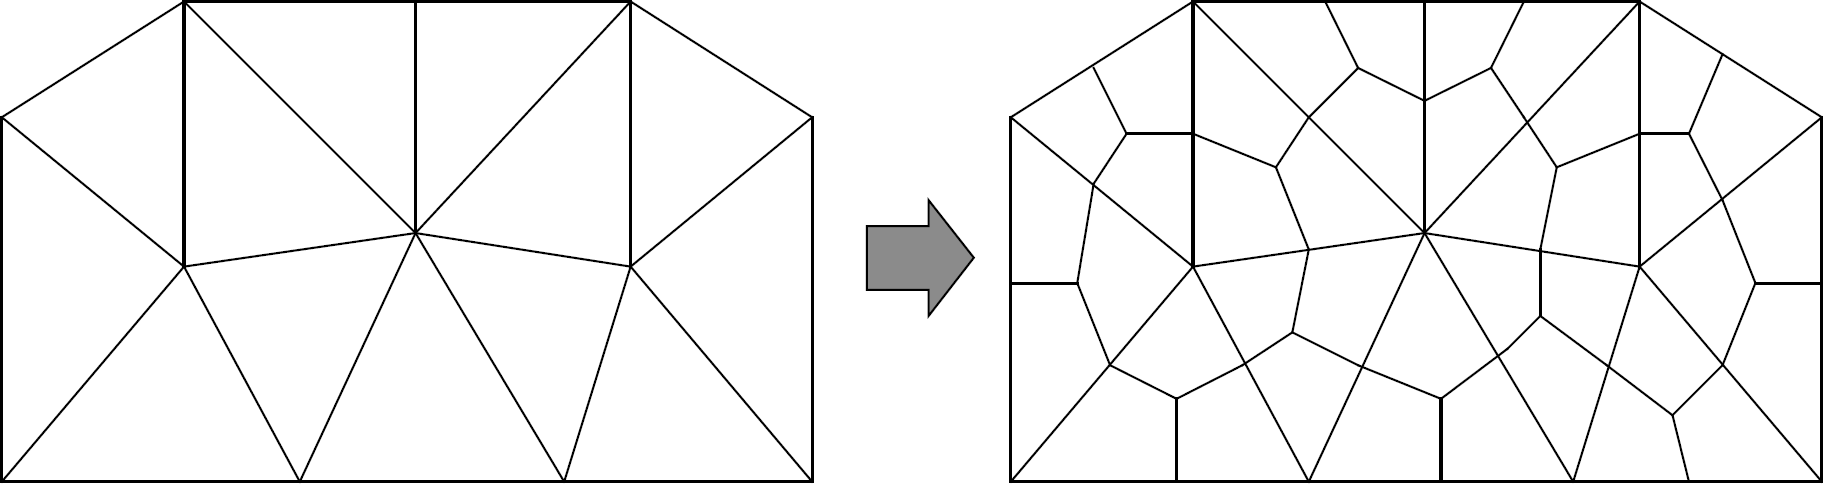
\includegraphics[scale=0.42]{images/tri_to_quad_1.png}
    \caption{Génération de maillage quadrilatéral par subdivision de chaque triangle en quatre quadrangles. Source : \cite{owen1998survey}.}
    \label{fig:tri_to_quad_1}
\end{figure}

Combinaison de triangles: il s'agit de convertir un maillage triangulaire en maillage quadrangulaire via des opérations sur la connectivité. Le mécanisme principal consiste à fusionner deux triangles originaux en un quadrilatère ; en substance, la conversion de maillage triangulaire en maillage quadrangulaire repose sur la mise en paire des triangles adjacents d'origine \cite{bommes2013quad} (voir figure \ref{fig:tri_to_quad_2}). La méthode de combinaison de triangles peut être améliorée si l'on fait attention à l'ordre dans lequel les triangles sont combinés \cite{owen1998survey}. L'algorithme définit dans \cite{lo1989generating} propose plusieurs procédures heuristiques pour l'ordre dans lequel les triangles pourraient être combinés. Il en résulte un maillage à dominante de quadrilatères contenant un nombre minimal de triangles. Dans \cite{owen1998quad}, les auteurs utilisent une approche d'avancée de front pour convertir les triangles en quadrilatères, mais parvient à réduire considérablement le nombre de noeuds irréguliers dans le maillage. Des échanges locaux d'arêtes sont effectués et des nœuds supplémentaires sont introduits afin d'assurer l'alignement avec la frontière et l'orthogonalité. Un nombre quelconque de triangles peut être supprimé pour créer un seul quadrilatère.

\begin{figure}[!h]
    \centering
    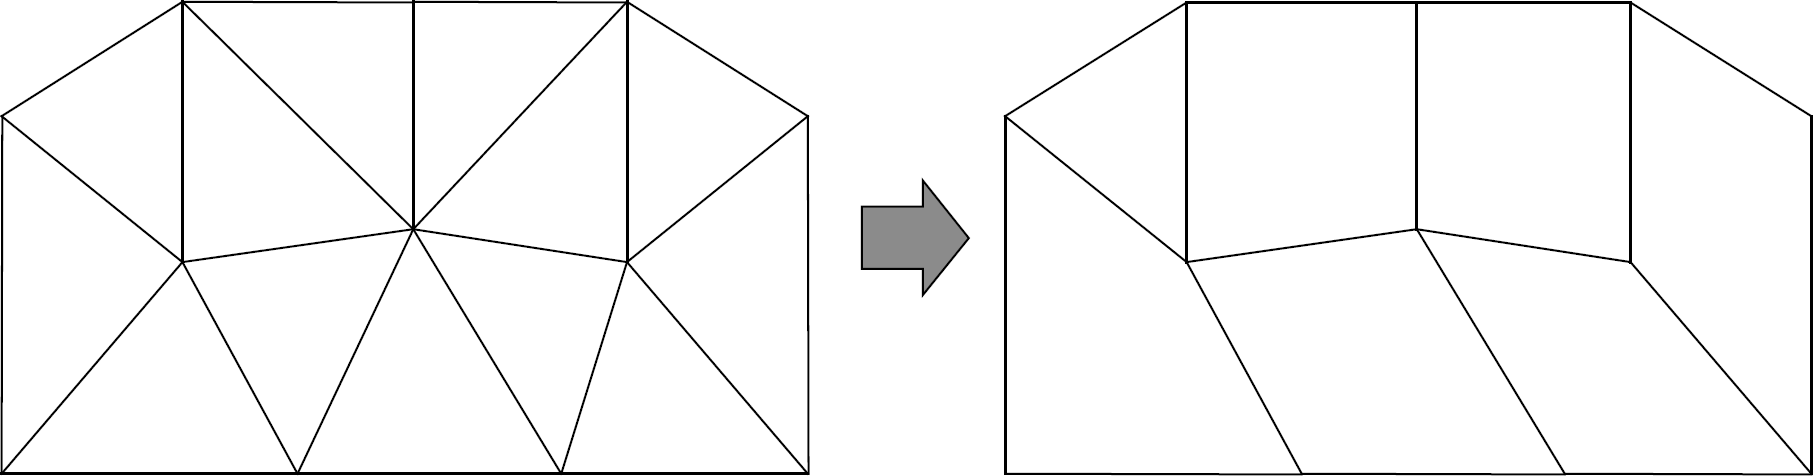
\includegraphics[scale=0.42]{images/tri_to_quad_2.png}
    \caption{Combinaison de triangles. Source : \cite{owen1998survey}.}
    \label{fig:tri_to_quad_2}
\end{figure}

D'autres algorithmes sont présenté dans \cite{bommes2013quad} tel que le SQuad \cite{gurung2011squad} conçu pour améliorer la représentation interne des maillages, mais  qui peut être utilisé pour définir un maillage quadrangulaire à partir d'un maillage triangulaire ou encore BlossomQuad \cite{remacle2012blossom} qui exploite un algorithme d'appariement parfait issu de l'optimisation combinatoire. Cependant, sa complexité algorithmique est quadratique par rapport au nombre d'éléments. Cela rend la méthode chronophage et principalement adaptée aux cas où l'optimalité du résultat est plus importante que le temps d'exécution.

\subsubsection{Méthodes basées sur la paramétrisation}

Les méthodes de paramétrisation sont des techniques utilisées en infographie et en géométrie numérique pour générer des mappages paramétrés d'une surface donnée sur un domaine plus simple, souvent un carré ou un rectangle, qui peut ensuite être utilisé pour générer des maillages quadrilatéraux. Ce processus est couramment utilisé dans la génération de maillages à diverses fins, notamment la modélisation 3D, la simulation et le rendu. Voici quelques méthodes de paramétrisation courantes pour générer des maillages quadrilatéraux:

\paragraph{Paramétrisation plane:} Il s'agit de la forme la plus simple de paramétrisation où la surface est projetée sur un domaine plan, tel qu'un carré ou un rectangle. Cela implique d'attribuer des coordonnées de texture 2D aux sommets du maillage. Cette méthode convient aux surfaces qui peuvent être approximativement aplaties sans distorsion significative.

\paragraph{Paramétrisation harmonique:} La paramétrisation harmonique vise à réduire la déformation entre une surface et le domaine paramétrique. Pour y parvenir, on résout une équation de Laplace sur la surface en imposant des conditions aux limites spécifiques basées sur le domaine paramétrique cible. Cette méthode est particulièrement efficace pour les surfaces de genre zéro (surfaces sans anses ni trous) et peut produire des paramétrisations de haute qualité. Elle a pour effet de préserver les détails de forme locaux, ce qui en fait un outil prisé dans les domaines de l'architecture et de l'ingénierie. Le processus implique les étapes suivantes :\\

\begin{enumerate}
    \item Sélection de points d'ancrage sur la surface, correspondant à des sommets dans le domaine paramétrique.\\
    \item Attribution de valeurs paramétriques fixes à ces points d'ancrage.\\
    \item Résolution de l'équation de Laplace pour le reste de la surface, de manière à obtenir une cartographie fluide qui minimise la déformation.
\end{enumerate}



\subsubsection{Superposition de grille régulière}

Ces méthodes débutent par la création d'un maillage dont la génération dans une étendue convenable autour de l'objet peut varier en complexité. L'algorithme introduit par Schneiders \cite{schneiders1996grid} (voir figure \ref{fig:superpo_grid_1}) déploie une grille structurée pour recouvrir une zone considérable autour de l'objet. La taille de chaque cellule dans cette grille peut être déterminée de manière arbitraire. Il ne reste plus qu'à ajuster la grille à la frontière de l'objet. Pour se faire, les éléments extérieurs à l'objet ou trop proches de sa frontière sont éliminés du maillage initial, laissant les cellules restantes pour former la structure de base du maillage. Ensuite, la zone entre la frontière de l'objet et le maillage initial est comblée en utilisant la technique d'isomorphisme. Cette technique implique que chaque nœud sur la frontière du maillage initial est associé à un nœud correspondant sur la frontière de l'objet, ce qui permet de remplir la région avec des éléments quadrilatéraux.

 \begin{figure}[!h]
    \centering
    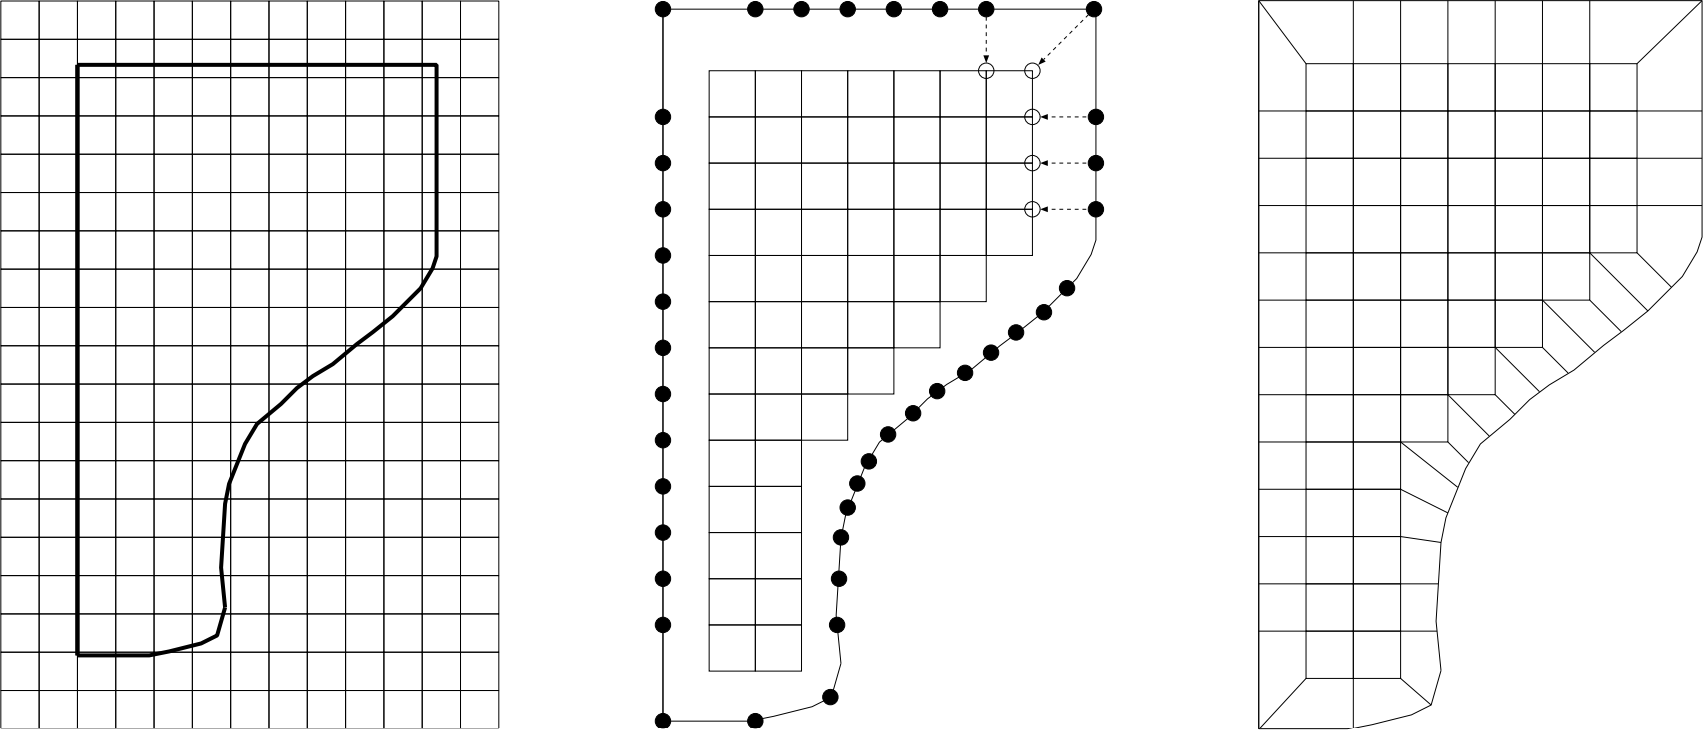
\includegraphics[scale=0.445]{images/superpo_grid_1.png}
    \caption{Méthode de superposition d'une grille régulière. Source : \cite{schneiders1996grid}.}
    \label{fig:superpo_grid_1}
\end{figure}

Dans \cite{taghavi1994automatic, ives1995geometric} les auteurs adoptent une autre méthode appelé méthode de projection  (voir figure \ref{fig:superpo_grid_2}). La grille initiale reste en place et les noeuds du maillage sont déplacés vers les arêtes de l'objet, de sorte que la frontière de l'objet soit entièrement recouverte par les arêtes du maillage. Le maillage est ensuite optimisé par un lissage laplacien.

 \begin{figure}[!h]
    \centering
    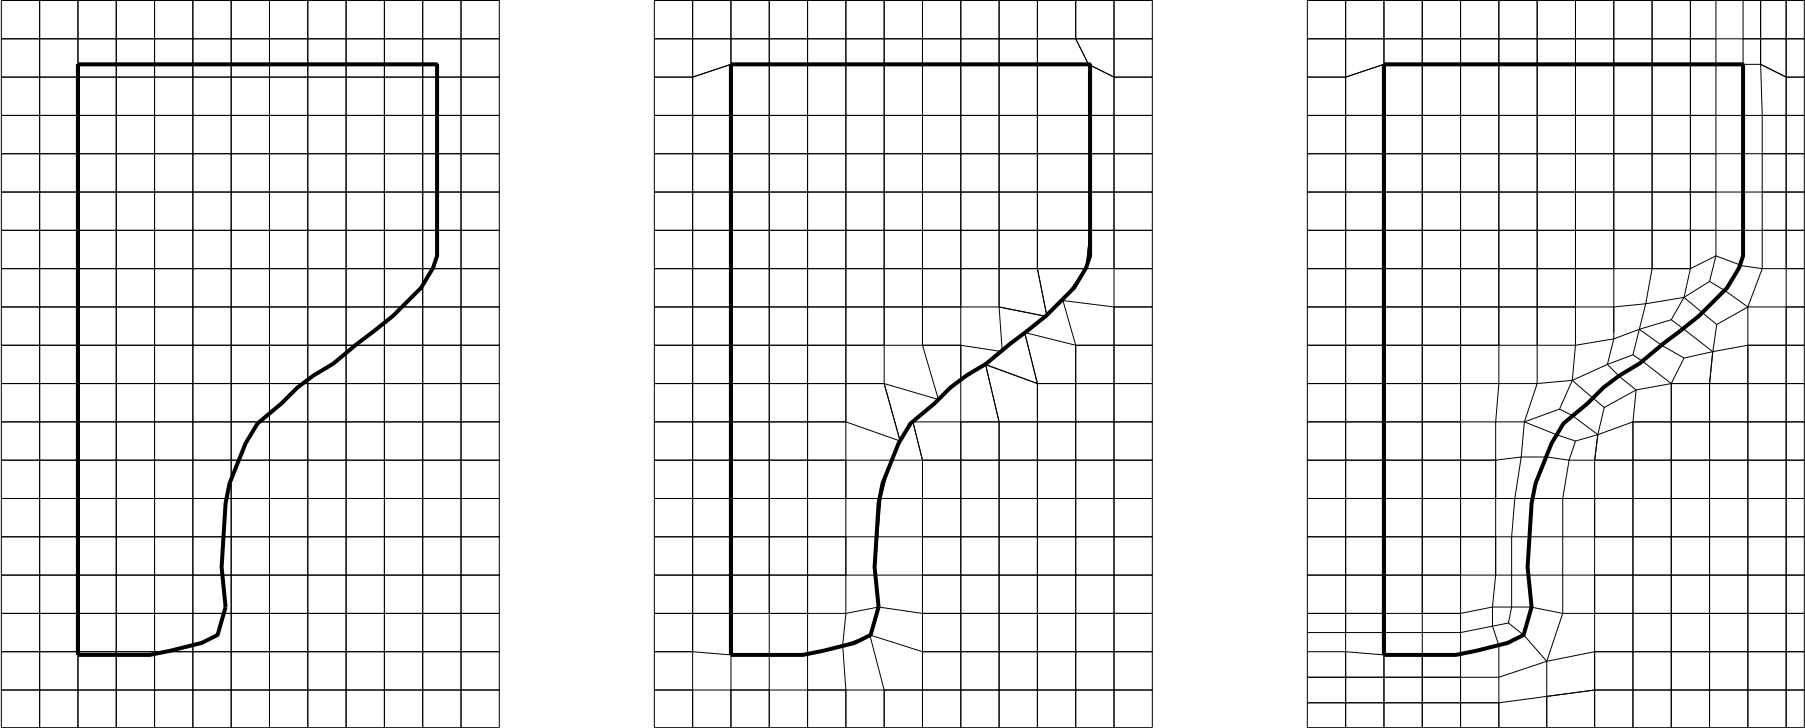
\includegraphics[scale=0.415]{images/superpo_grid_2.png}
    \caption{Méthode de projection. Source : \cite{schneiders1996grid}.}
    \label{fig:superpo_grid_2}
\end{figure}

\subsubsection{Méthode de l'axe médian}

La méthode de l'axe médian, également connue sous le nom de méthode de squelettisation, est une technique utilisée en infographie et en géométrie numérique pour générer des maillages quadrilatéraux à partir de formes complexes. Cette méthode vise à trouver une représentation simplifiée de la forme d'entrée en identifiant le "squelette" central ou l'"axe médian" de la forme. Cette méthode a d'abord été conçue par Nackman et Srinivasan \cite{nackman1989method}. Ils ont remarqué que l'axe médian présentait une décomposition naturelle bien définie de la surface et l'ont utilisé sans modifications pour diviser la surface en blocs. Quelques règles supplémentaires pour fusionner les blocs produits ont été élaborées pour améliorer l'adéquation de la décomposition. Une méthode améliorée a été proposée par Tam et Armstrong \cite{tam19912d} qui produit des décompositions de meilleure qualité.

Voici un aperçu de la manière dont fonctionne la méthode de l'axe médian pour la génération de maillages quadrilatéraux :\\

\begin{itemize}
    \item  Géométrie d'entrée : on commence avec une forme polygonale complexe et irrégulier. Cette forme peut représenter la limite d'un objet en 2D ou la surface d'un objet en 3D.\\

    \item Diagramme de Voronoi : la première étape consiste à calculer le diagramme de Voronoi de la forme d'entrée. Le diagramme de Voronoi divise l'espace autour de chaque point (ou sommet) de la forme en régions. Chaque région contient tous les points qui sont plus proches d'un sommet particulier que de tout autre sommet de la forme. Ces régions sont appelées cellules de Voronoi.\\

    \item Squelettisation (voir Figure \ref{fig:median_axis}): l'axe médian est essentiellement le dual du diagramme de Voronoi. Pour obtenir l'axe médian, on trouve les centres des cercles circonscrits pour chaque cellule de Voronoi. L'axe médian représente le "squelette" central de la forme d'entrée, qui capture ses principales caractéristiques et sa connectivité.\\

    \item Suppression des arêtes : dans l'axe médian, il y a souvent de nombreuses branches et arêtes qui ne sont pas pertinentes pour le maillage quadrilatéral souhaité. Ces branches superflues doivent parfois être supprimées ou élaguées pour simplifier le squelette tout en préservant les caractéristiques essentielles de la forme.\\

    \item Génération du maillage quadrilatéral : une fois que vous avez l'axe médian a été simplifié, on génère des éléments quadrilatéraux en connectant des paires de points proches sur le squelette. Ces connexions doivent former un réseau d'éléments quadrilatéraux qui approximent la forme d'entrée.\\

    \item Affinement : en fonction de la qualité et de la régularité du maillage quadrilatéral initial, on peut effectuer des étapes d'affinement. Cela peut impliquer le lissage du maillage, la redistribution des sommets ou l'optimisation de la disposition des quadrilatères pour répondre à des critères spécifiques tels que l'uniformité ou la préservation de la forme.\\
\end{itemize}

La méthode de l'axe médian est puissante pour la génération de maillages quadrilatéraux, en particulier pour les formes avec des limites irrégulières ou des caractéristiques complexes. Elle offre une manière de représenter la topologie de la forme de manière simplifiée et structurée. Cependant, l'efficacité de la méthode dépend de la qualité de la squelettisation initiale et des étapes ultérieures prises pour affiner et optimiser le maillage quadrilatéral. Divers algorithmes et techniques existent pour chaque étape du processus, et le choix des méthodes peut varier en fonction des exigences spécifiques de l'application.

\begin{figure}
    \centering
    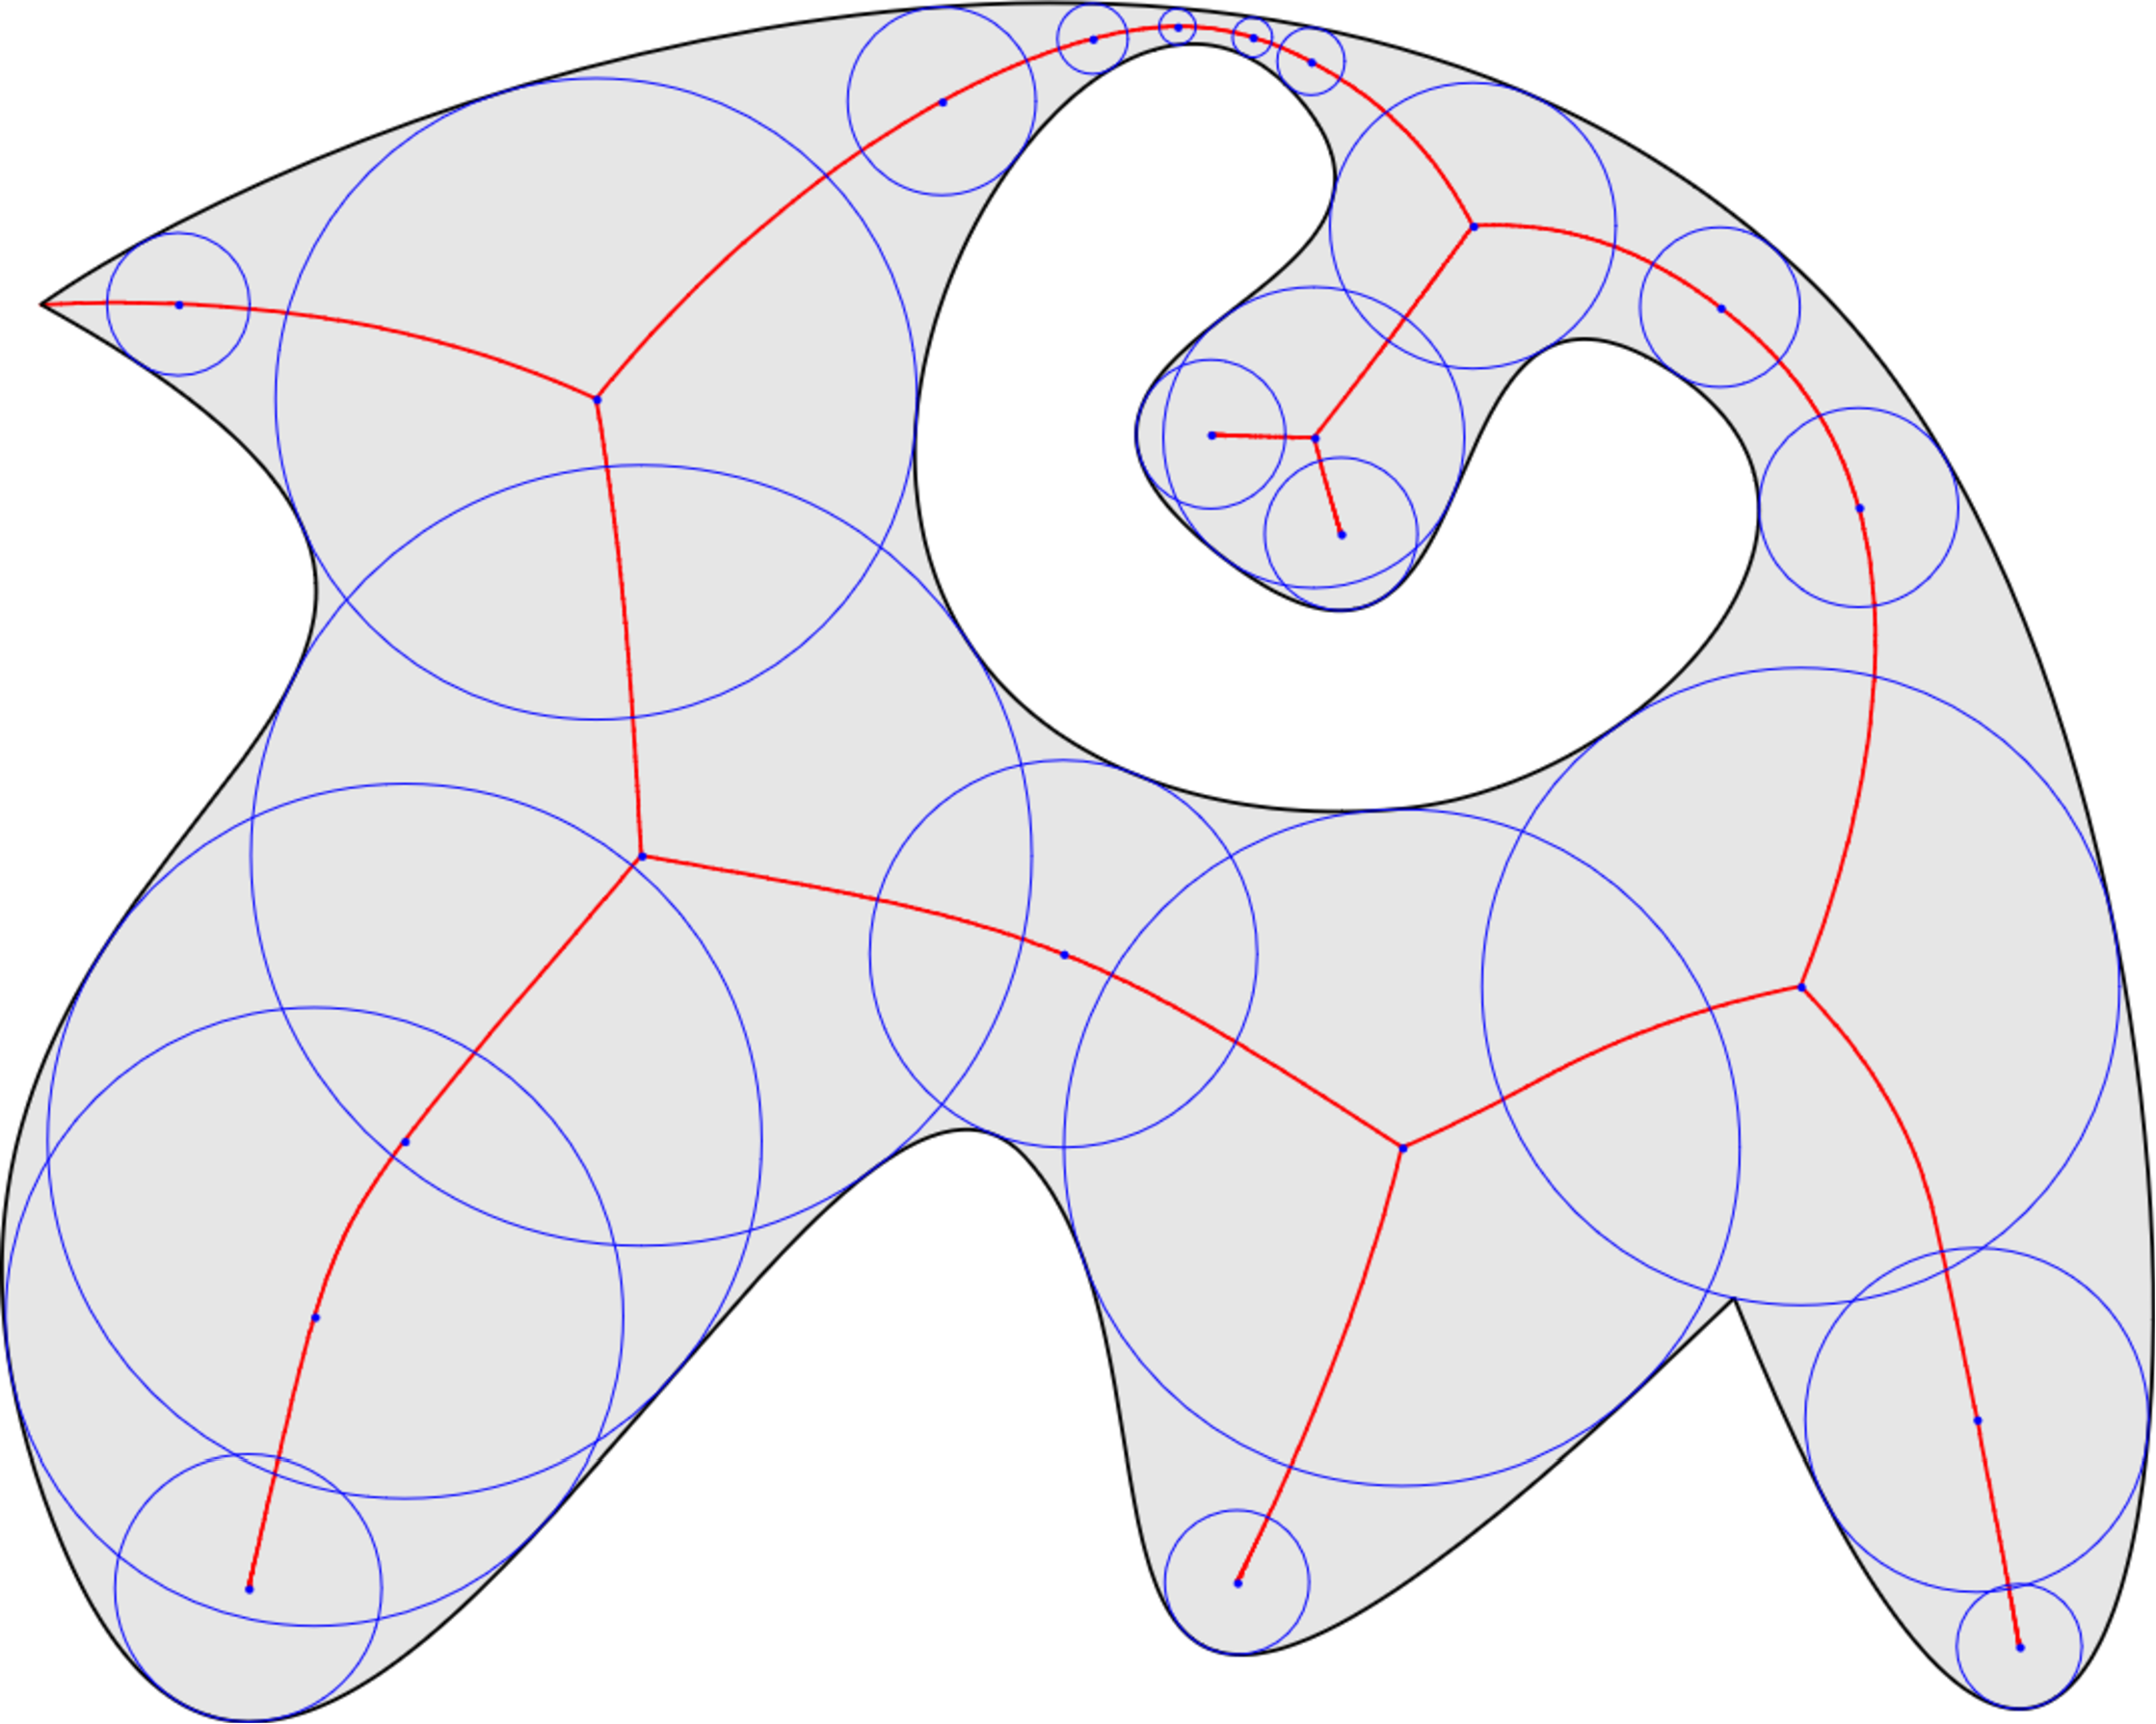
\includegraphics[scale=0.3]{images/median_axis.pdf}
    \caption{Construction de l'axe médian. Source: \cite{de2009fast}}
    \label{fig:median_axis}
\end{figure}

\subsubsection{Approches basées sur l'avancée de fronts}

Ces méthodologies s'apparentent à celles abordées pour la formation de maillages triangulaires. Une première méthode débute avec un maillage triangulaire puis définit des ensembles de fronts le long des arêtes de triangles de la frontière du domaine. Les triangles sont systématiquement combinés à ces fronts, progressant vers l'intérieur de la zone. Le front agit comme une division entre les quadrilatères déjà formés et les triangles qui doivent encore être combinés. Cette technique garantit un maillage entièrement quadrilatéral, à condition que le nombre initial d'arêtes de la frontière soit pair \cite{owen1999q}. D'autres méthodes se basent sur une approche directe. Le pavage présenté par Blacker et Stephenson \cite{blacker1991paving} consiste à former des rangées complètes d'éléments à partir de la frontière tout en progressant vers l'intérieur. White and Kinney ont avancé des améliorations à l'algorithme de pavage en préconisant l'insertion individuelle d'éléments plutôt que la création de rangées complètes \cite{white1997redesign}. Une alternative intéressante aux méthodes de pavage traditionnelle est l'algorithme Q-Morph. Il s'agit d'une méthode indirecte donc basée sur un maillage triangulaire initial permettant de maintenir des rangées d'éléments bien alignés et de réduire le nombre de nœuds irréguliers internes. Les différentes étapes de cette méthode sont les suivantes \cite{owen1999q}:\\

\begin{itemize}
    \item Maillage initial: initialement, la surface est triangulée en utilisant n'importe quelle méthode de triangulation de surface. Ce maillage devrait intégrer toute information de dimensionnement ou d'adaptativité. Le dimensionnement local pour le maillage quadrilatéral final suivra de près celui du maillage triangulaire.\\

    \item Définition du Front: le front initial est établi à partir des arêtes de la triangulation. Toute arête qui est adjacente à un seul triangle fait partie du front initial.\\

    \item Classification des arêtes de front: chaque arête dans le front est catégorisée en fonction de son état qui détermine comment l'arête sera finalement utilisée pour former un quadrilatère. Les états des arêtes frontales sont déterminés par les angles entre les arêtes adjacentes. Ces arêtes seront mises à jour et réorganisées au fur et à mesure que l'algorithme progresse.\\

    \item Traitement des arêtes frontales: chaque arête frontale est traitée individuellement pour construire un nouveau quadrilatère en utilisant les triangles du maillage triangulaire (voir Figure \ref{fig:step_front_advancing}).

    \begin{figure}[!h]
    \centering
    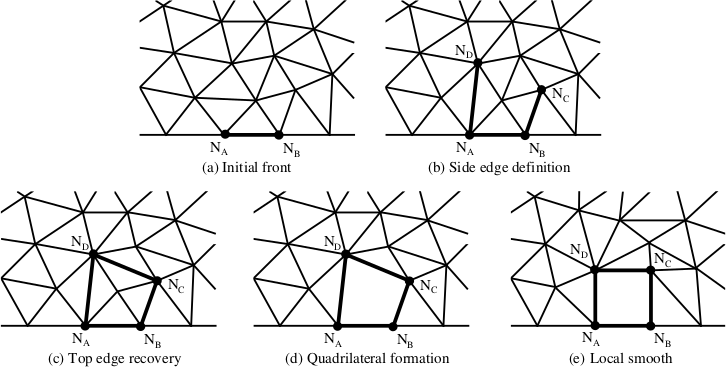
\includegraphics[scale=0.62]{images/step_front_advancing.png}
    \caption{Illustration du processus de génération d'un quadrilatère à partir d'une arête frontale. Source : \cite{owen1999q}.}
    \label{fig:step_front_advancing}
    \end{figure}

    \item Nettoyage topologique: la qualité des éléments est améliorée en effectuant des transformations locales sur les quadrilatères dans le but d'améliorer les valences individuelles des arêtes au niveau des nœuds du maillage.\\

    \item Lissage: une dernière étape de lissage est réalisée pour améliorer davantage la qualité des éléments.\\
\end{itemize}


\section{Maillages quadrilatéraux à partir de champs de croix}

Une méthode de génération de maillages quadrilatéraux intéressante repose sur les \emph{champs de croix}. Un champ de croix sur un domaine est une structure de champ qui attribue une \emph{croix} à presque chaque point du domaine, où une croix est un ensemble de vecteurs du fibré tangent. Elle est constitué d'un vecteur donné et de ses rotations avec un angle de $k\displaystyle\frac{\pi}{2}$, où $k \in \llbracket 0,3\rrbracket$. Les champs de croix sont utilisés pour la première fois dans les applications de graphisme informatique pour contrôler la mise en correspondance de surface pour le rendu non photoréaliste, la synthèse de textures et le ramaillage \cite{ray2008n, bommes2009mixed, nieser2011cubecover}.\\

\paragraph{Lien entre les champ de croix et les maillages quadrilatéraux:} une astuce particulièrement ingénieuse consiste à exploiter les lignes de champ d'un vecteur pour définir les quadrilatères d'un maillage quadrilatéral sur un domaine donné. Toutefois, pour que cela fonctionne, il est impératif de garantir que ces lignes de champ ne se croisent que sous un angle de $\frac{\pi}{2}$. C'est pourquoi l'utilisation d'un champ spécifique constitué de croix en chaque point du domaine est cruciale. L'avantage des champs de croix est de pouvoir représenter les caractéristiques des quadrilatères en deux dimensions. Dans \cite{beaufort2017computing}, les auteurs montrent que les sommets non réguliers d'un maillage quadrilatéral (les sommets qui ne sont pas adjacents à exactement quatre voisins) correspondent précisément aux points critiques d'un champ de croix. Ces points critiques du champ de croix peuvent également être liés à la caractéristique d'Euler de la surface maillée via la formule de Poincaré suivante:
$$
\sum_i index(x_i)=\chi,
$$
où $\chi=V-E+F$ désigne la caractéristique d'Euler, avec $V$ le nombre de sommets, $E$ le nombre d'arêtes et $F$ le nombre de faces.\\

Les méthodes de génération de maillage basées sur les champs de croix se décomposent en deux étapes principales à savoir la génération du champ de croix puis la construction du maillage quadrilatéral correspondant.

\paragraph{Géneration du champ de croix:} l'idée est de calculer un champ de croix le plus lisse possible afin de minimiser les variations brusques de l'orientation des quadrangles. 

Lorsqu'on aborde le cas d'une surface, l'approximation la plus optimale est obtenue en alignant les éléments selon les directions principales de courbure. Ainsi, il est préférable de générer des champs de croix qui suivent ces directions. Cette approche a été mise en œuvre dans des travaux tels que \cite{alliez2003anisotropic, marinov2004direct, kalberer2007quadcover}. Ce choix méthodologique présente l'avantage de créer des champs de croix attrayants qui s'harmonisent avec les propriétés inhérentes de la surface grâce à une méthode simple, ce qui a pour résultat que les singularités se forment naturellement aux points ombilicaux. Cependant, il convient de noter qu'il existe des zones étendues où la courbure normale se rapproche des valeurs de courbure principales, engendrant une définition moins précise du champ de croix \cite{fogg2015automatic}.

Un autre critère necessaire pour les simulations est le respect de la frontiere du domaine lors de la discritisation. Pour se faire, il est necessaire de prendre en compte des contraintes d'alignements par rapport aux frontieres des elements quadrangulaires. Généralement un ensemble d'arêtes d'un maillage triangulaire ou d'une géométrie de CAO est utilisé comme condition aux limites afin de générer un champ de croix aligné avec ces  arêtes. c'est ce qui est mis en oeuvre dans \cite{kowalski2013pde, palacios2007rotational} où un champ vectoriel de représentation est résolu via une équation de la chaleur avec des conditions aux limites de Dirichlet donné par la normale aux bords. Cette méthode ne peut cependant pas traiter facilement les surfaces courbes et elle n'est pas adaptée pour s'ajuster aux tailles et directions d'élements cibles \cite{fogg2015automatic}. \cite{bommes2009mixed} proposent une formulation d`optimisation linéaire à variables mixtes, résolue à l'aide d'un solveur adaptatif. Des contraintes directionnelles éparses permettent de déterminer automatiquement le nombre approprié, le type et la position des singularités. Dans \cite{bunin2008towards}, Bunin résoud directement un probleme de Poisson inverse avec une distribution de sources ponctuelles représentant les irrégularité du maillage. La méthode est attrayante d'un point de vue théorique et montre des résultats impressionnants. Cependant, elle semble contenir des étapes nécessitant un réglage minutieux et des sensibilités élevées aux erreurs numériques sont rapportées pour les problèmes avec un grand nombre de singularités \cite{fogg2015automatic}.


\paragraph{Génération d'un maillage correspondant au champ de croix calculé:}

Une stratégie initiale pour générer des maillages quadrilatéraux à partir de champs de repères croisés consiste en la paramétrisation. Cette méthode implique la création d'une transformation du domaine à mailler vers un espace paramétrique, où l'application d'une grille régulière au domaine transformé devient possible. Inverser cette transformation permet alors de dériver un maillage quadrilatéral du domaine, aligné sur ses contours. L'avantage majeur de cette approche réside dans sa capacité à gérer des discontinuités dans la transformation, ce qui en fait une méthode adaptée pour traiter des singularités \cite{reberol2018maillages}. Il existe des algorithmes robustes basés sur des paramétrisations globales \cite{ray2006periodic, kalberer2007quadcover, myles2014robust, campen2015quantized}. L'élément clé de ces algorithmes est la décomposition du domaine en des cartes de forme quadrilatère en découpant le domaine le long d'un graphe en suivant par exemple les lignes de champ du champ de croix. Ainsi dans \cite{ray2006periodic}, les auteurs paramétrisent des surfaces de genre arbitraire avec des fonctions de potentiel périodiques guidées par deux champs vectoriels d'entrée orthogonaux. Cela conduit à une paramétrisation continue à l'exception des points singuliers sur la surface. Ces régions singulières sont détectées et reparamétrées par la suite. L'algorithme QuadCover \cite{kalberer2007quadcover} calcule automatiquement une paramétrisation globale dont les lignes paramétriques sont guidées par le champ de croix. La méthode génère des maillages quadrilatéraux de bonne qualité avec des éléments de petites tailles mais gère difficilement des tailles de maillages grossières.

Outre la paramétrisation, une autre méthode consiste à générer une partition du domaine en utilisant le champ de croix.  Dans \cite{kowalski2013pde}, les auteurs construisent ce partitionnement en traçant des lignes de séparation à travers le champ croisé. Les champs croisés sont utilisés pour capturer les caractéristiques d'orientation des quadrilatères, permettant ainsi la génération d'une partition bien définie du domaine en sous-domaines. Il est ensuite nécessaire de résoudre un problème d'assignation d'intervalles pour le maillage quadrilatère consistant à attribuer à chaque courbe le nombre d'arêtes (intervalles) en lesquelles elle doit être subdivisée, de manière à ce que chaque surface  puisse être maillée \cite{hohring1997mesh, mitchell2000high, mitchell2014simple}. Par exemple, mailler une surface rectangulaire avec des quadrilatères nécessite que les courbes sur les côtés opposés contiennent exactement le même nombre d'arêtes.


\section{Objectif de la thèse}
\label{thesis_target}

L'objectif de cette thèse est d'amener de nouvelles solutions pour gagner en performance lors de résolutions numériques d'équations aux dérivées partielles (en particulier pour l'électromagnétisme, la mécanique des fluides, l'élasticité, etc.).

Dans un premier temps, nous nous intéressons à la possibilité de construire un maillage quadrilatéral à partir d'un champ de croix fournit par un utilisateur. En effet, les champs de croix générer en propageant la normale extérieur à l'intérieur du domaine \cite{kowalski2013pde} produisent une distribution de singularités pouvant conduire à un partitionnement invalide ou non souhaité. Un problème notable survient dans les domaines extrêmement étirés, tandis qu'une autre préoccupation concerne les formes de partitionnement qui entraînent des tailles de cellules très non uniformes (voir figure \ref{fig:dom_etire_mesh_inhomogene}).

\begin{figure}[!h]
    \centering
    %\includegraphics[scale=0.5]{img/cercle non_homogene.pdf}
    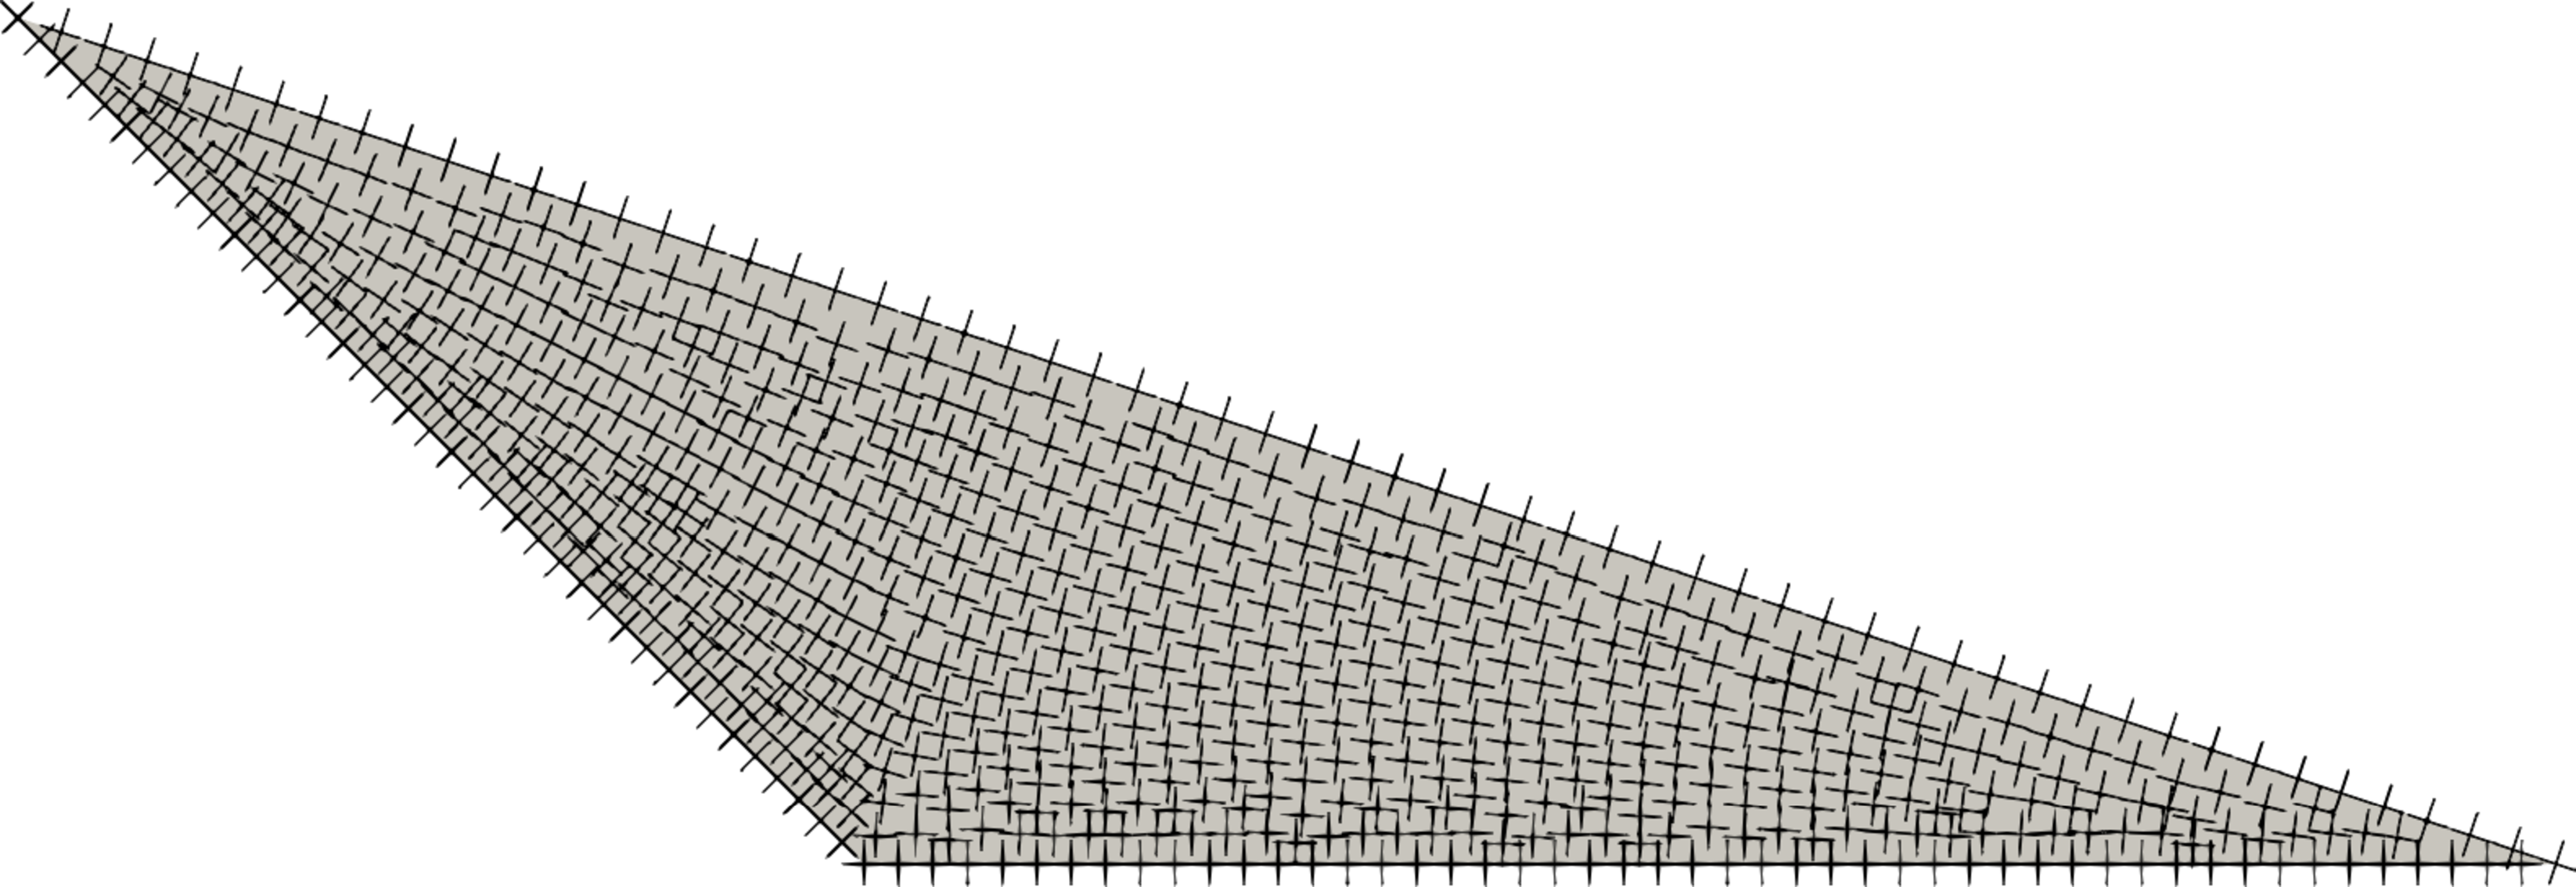
\includegraphics[scale=0.189]{images/stretch.pdf}
    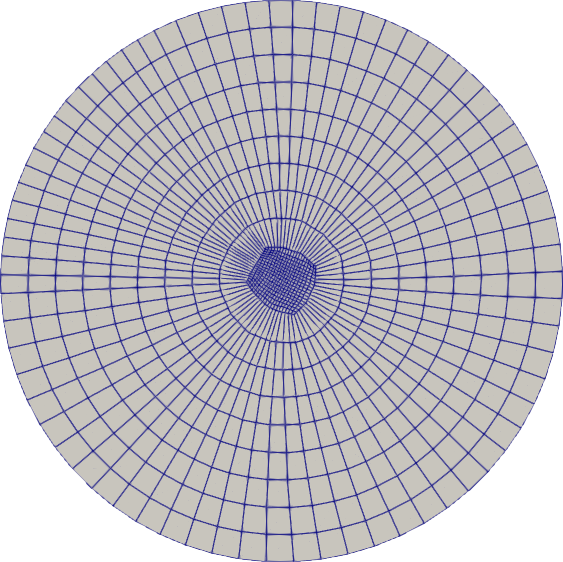
\includegraphics[scale=0.245]{images/new_cercle.png}
    \caption{Gauche: Champ de croix sur un domaine étiré; Droite: Maillage non-homogène d'un disque.}
    \label{fig:dom_etire_mesh_inhomogene}
\end{figure}

Pour surmonter ces problèmes, il est essentiel de focaliser notre attention sur le contrôle à la fois du type et de l'emplacement des points singuliers dans le champ croisé. À cet égard, Jezdimirović et al. \cite{jezdimirovic2021quad} ont présenté un algorithme qui repose sur un modèle de singularité spécifié par l'utilisateur en entrée, pouvant inclure des singularités de grande valence. De même, Alexis Macq et al. \cite{macq2020ginzburg} ont élaboré une formulation basée sur l'énergie de Ginzburg-Landau, qui permet d'imposer des singularités internes en les substituant par de petits trous pratiqués dans le domaine. Dans le cadre de cette thèse, nous explorons une approche qui prend racine dans la sélection d'un champ de croix répondant à un ensemble spécifique de propriétés. Ensuite, nous cherchons à aligner ce champ par rapport aux frontières du domaine de calcul. Par la suite nous élargissons cette approche aux domaines non simplement connexes, dans le but de pouvoir tenir compte des situations où le domaine est constitué de plusieurs matériaux distincts (multi-matériau).

Lors des simulations numériques, prendre en compte les conditions aux limites est une étape fondamentale. Pour ce faire, il est impératif d'introduire des points de passage dans le maillage, créant ainsi des segments de frontières qui correspondent à la localisation de ces conditions aux limites dans la structure du maillage. Dans cette optique, notre intention est d'enrichir le processus mentionné précédemment, qui concerne le champ croisé, en intégrant la prise en compte de ces points de passage, qui se manifestent sous forme de singularités de bord.

Nous étendons enfin cette approche aux surfaces courbes, et à l'instar de \cite{viertel2019approach}, nous établissons un cadre théorique pour analyser la régularité des champs croisés, tout en présentant une série d'opérations qui facilitent leur manipulation.

\section{Organisation du manuscrit}
Ce mémoire est organisé de la manière suivante:\\\\
Le \textbf{\color{blue!50!black}{Chapitre \ref{chap:theoritical}}} formalise la notion de champ de croix dans le but de la comprendre en vue de l'utiliser comme point d'entrée d'une méthode de génération de maillage quadrilatéral. Nous abordons les notions d'angles, de points singuliers, d'indice, et de ligne de champ d'un champ de croix. L'intégration d'une ligne de champ à partir d'un point singulier est soigneusement étudiée, tout comme le comportement local du champ de croix au voisinage d'un point singulier. Ensuite, nous mettons en place un processus de partitionnement ainsi que les hypothèses permettant à ce partitionnement de conduire à une décomposition d'un domaine à quatre côtés. Sur cette base, nous présentons un processus dit \emph{d'alignement}, permettant de définir un champ de croix puis de l'adapter à un domaine en vue de générer à partir de ce dernier un maillage quadrilatéral. Ce processus est initialement présenté pour des domaines simplement connexes puis généralisé à des domaines non-simplement connexes.\\\\
Dans le \textbf{\color{blue!50!black}{Chapitre \ref{chap:alorithme}}}, nous abordons la discrétisation de la méthode présentée dans le  \ref{chap:theoritical}. Pour ce faire, nous définissons une représentation discrète du champ de croix sur un maillage triangulaire. Cette représentation nous permet de retrouver une version discrète des notions présentées dans le cadre continu. Ainsi, nous pouvons mettre en œuvre une version discrète du processus de partitionnement permettant d'aboutir à une décomposition du maillage triangulaire. Nous montrons alors qu'une telle décomposition convergera lorsqu'on raffine le maillage vers une décomposition en régions de quatre côtés, qui se trouve être la décomposition du domaine continu.\\\\
Dans le \textbf{\color{blue!50!black}{Chapitre \ref{chap:surface_courbe}}}, nous étendons les approches développées au cas des surfaces courbes dans l'espace. La difficulté principale dans ce cadre réside dans l'absence de référence globale pour le domaine considéré. Nous reprenons le résultat permettant de garantir le bon fonctionnement du partitionnement, puis nous retrouvons le processus d'alignement dans le cas des domaines non simplement connexes. Une approche alternative est présentée, consistant à créer un repère global à partir de l'équation de la chaleur vectorielle. Enfin, nous abordons, comme dans le chapitre \ref{chap:alorithme}, l'analyse de convergence du maillage généré.

\section{Communications issues de la thèse}

Les travaux de recherche effectués ont mené aux communications suivantes:

\subsubsection{Article soumis}

\subsubsection{Proceeding}

\subsubsection{Communications orales dans des conférences internationales}

\begin{itemize}
    \item \textit{Quadrilateral mesh create from a given cross field}, 10th International Conference on Curves and Surfaces, Arcachon, France, 20-24 Juin 2022.\\
    \item \textit{Quadrilateral mesh of non-simply connected domain and non-planar surfaces from a given cross-field}, The SIAM International Meshing Roundtable Workshop 2023 (SIAM IMR 2023), Amsterdam, Netherlands, 06-09 Mars 2023.
\end{itemize}

\subsubsection{Communications orales dans des conférences nationales}

\begin{itemize}
    \item \textit{Génération de maillages quadrilatéraux à partir de champs de croix donnés}, Journées Ondes du Sud-Ouest 2023 (JOSO 2023), Toulouse, France, 14-16 Mars 2023.\\
    \item \textit{Méthode de maillage en quadrilatères par résolution d'EDP}, Laboratoire de Mathématiques Appliquées à l'Aéronautique et au Spatial (LMA2S), Toulouse, France, Mars 2021.
\end{itemize}



\subsubsection{Communications dans des séminaires doctorants}


\subsubsection{Logiciels}


